\documentclass[oneside]{book}

\usepackage{amsmath, amsthm, amssymb, amsfonts}
\usepackage{thmtools}
\usepackage{graphicx}
\usepackage{setspace}
\usepackage{geometry}
\usepackage{float}
\usepackage{hyperref}
\usepackage[utf8]{inputenc}
\usepackage[english]{babel}
\usepackage{framed}
\usepackage[dvipsnames]{xcolor}
\usepackage{environ}
\usepackage{tcolorbox}
\tcbuselibrary{theorems,skins,breakable}

%打中文需要以下packages
\usepackage{xeCJK} 
\setCJKmainfont[BoldFont={cwTeXHeiBold}, ItalicFont={FandolSong}]{cwTeXMing} %Overleaf 中文字型設定
\XeTeXlinebreaklocale "zh"
\XeTeXlinebreakskip = 0pt plus 1pt %這兩行一定要加,中文才能自動換行


\setstretch{1.2}
\geometry{
    textheight=9in,
    textwidth=5.5in,
    top=1in,
    headheight=12pt,
    headsep=25pt,
    footskip=30pt
}

% Variables
\def\notetitle{MATH 101}
\def\noteauthor{
    \textbf{Professor} \\ 
    {\LaTeX} by Joe\\
    University}
\def\notedate{Semester}

% The theorem system and user-defined commands
% Theorem System
% The following boxes are provided:
%   Definition:     \defn 
%   Theorem:        \thm 
%   Lemma:          \lem
%   Corollary:      \cor
%   Proposition:    \prop   
%   Claim:          \clm
%   Fact:           \fact
%   Proof:          \pf
%   Example:        \ex
%   Remark:         \rmk (sentence), \rmkb (block)
% Suffix
%   r:              Allow Theorem/Definition to be referenced, e.g. thmr
%   p:              Add a short proof block for Lemma, Corollary, Proposition or Claim, e.g. lemp
%                   For theorems, use \pf for proof blocks

% Definition
\newtcbtheorem[number within=section]{mydefinition}{Definition}
{
    enhanced,
    frame hidden,
    titlerule=0mm,
    toptitle=1mm,
    bottomtitle=1mm,
    fonttitle=\bfseries\large,
    coltitle=black,
    colbacktitle=green!20!white,
    colback=green!10!white,
}{defn}

\NewDocumentCommand{\defn}{m+m}{
    \begin{mydefinition}{#1}{}
        #2
    \end{mydefinition}
}

\NewDocumentCommand{\defnr}{mm+m}{
    \begin{mydefinition}{#1}{#2}
        #3
    \end{mydefinition}
}

% Theorem
\newtcbtheorem[use counter from=mydefinition]{mytheorem}{Theorem}
{
    enhanced,
    frame hidden,
    titlerule=0mm,
    toptitle=1mm,
    bottomtitle=1mm,
    fonttitle=\bfseries\large,
    coltitle=black,
    colbacktitle=cyan!20!white,
    colback=cyan!10!white,
}{thm}

\NewDocumentCommand{\thm}{m+m}{
    \begin{mytheorem}{#1}{}
        #2
    \end{mytheorem}
}

\NewDocumentCommand{\thmr}{mm+m}{
    \begin{mytheorem}{#1}{#2}
        #3
    \end{mytheorem}
}

% Lemma
\newtcbtheorem[use counter from=mydefinition]{mylemma}{Lemma}
{
    enhanced,
    frame hidden,
    titlerule=0mm,
    toptitle=1mm,
    bottomtitle=1mm,
    fonttitle=\bfseries\large,
    coltitle=black,
    colbacktitle=violet!20!white,
    colback=violet!10!white,
}{lem}

\NewDocumentCommand{\lem}{m+m}{
    \begin{mylemma}{#1}{}
        #2
    \end{mylemma}
}

\newenvironment{lempf}{
	{\noindent{\it \textbf{Proof for Lemma}}}
	\tcolorbox[blanker,breakable,left=5mm,parbox=false,
    before upper={\parindent15pt},
    after skip=10pt,
	borderline west={1mm}{0pt}{violet!20!white}]
}{
    \textcolor{violet!20!white}{\hbox{}\nobreak\hfill$\blacksquare$} 
    \endtcolorbox
}

\NewDocumentCommand{\lemp}{m+m+m}{
    \begin{mylemma}{#1}{}
        #2
    \end{mylemma}

    \begin{lempf}
        #3
    \end{lempf}
}

% Corollary
\newtcbtheorem[use counter from=mydefinition]{mycorollary}{Corollary}
{
    enhanced,
    frame hidden,
    titlerule=0mm,
    toptitle=1mm,
    bottomtitle=1mm,
    fonttitle=\bfseries\large,
    coltitle=black,
    colbacktitle=orange!20!white,
    colback=orange!10!white,
}{cor}

\NewDocumentCommand{\cor}{+m}{
    \begin{mycorollary}{}{}
        #1
    \end{mycorollary}
}

\newenvironment{corpf}{
	{\noindent{\it \textbf{Proof for Corollary.}}}
	\tcolorbox[blanker,breakable,left=5mm,parbox=false,
    before upper={\parindent15pt},
    after skip=10pt,
	borderline west={1mm}{0pt}{orange!20!white}]
}{
    \textcolor{orange!20!white}{\hbox{}\nobreak\hfill$\blacksquare$} 
    \endtcolorbox
}

\NewDocumentCommand{\corp}{m+m+m}{
    \begin{mycorollary}{}{}
        #1
    \end{mycorollary}

    \begin{corpf}
        #2
    \end{corpf}
}

% Proposition
\newtcbtheorem[use counter from=mydefinition]{myproposition}{Proposition}
{
    enhanced,
    frame hidden,
    titlerule=0mm,
    toptitle=1mm,
    bottomtitle=1mm,
    fonttitle=\bfseries\large,
    coltitle=black,
    colbacktitle=yellow!30!white,
    colback=yellow!20!white,
}{prop}

\NewDocumentCommand{\prop}{+m}{
    \begin{myproposition}{}{}
        #1
    \end{myproposition}
}

\newenvironment{proppf}{
	{\noindent{\it \textbf{Proof for Proposition.}}}
	\tcolorbox[blanker,breakable,left=5mm,parbox=false,
    before upper={\parindent15pt},
    after skip=10pt,
	borderline west={1mm}{0pt}{yellow!30!white}]
}{
    \textcolor{yellow!30!white}{\hbox{}\nobreak\hfill$\blacksquare$} 
    \endtcolorbox
}

\NewDocumentCommand{\propp}{+m+m}{
    \begin{myproposition}{}{}
        #1
    \end{myproposition}

    \begin{proppf}
        #2
    \end{proppf}
}

% Claim
\newtcbtheorem[use counter from=mydefinition]{myclaim}{Claim}
{
    enhanced,
    frame hidden,
    titlerule=0mm,
    toptitle=1mm,
    bottomtitle=1mm,
    fonttitle=\bfseries\large,
    coltitle=black,
    colbacktitle=pink!30!white,
    colback=pink!20!white,
}{clm}


\NewDocumentCommand{\clm}{m+m}{
    \begin{myclaim*}{#1}{}
        #2
    \end{myclaim*}
}

\newenvironment{clmpf}{
	{\noindent{\it \textbf{Proof for Claim.}}}
	\tcolorbox[blanker,breakable,left=5mm,parbox=false,
    before upper={\parindent15pt},
    after skip=10pt,
	borderline west={1mm}{0pt}{pink!30!white}]
}{
    \textcolor{pink!30!white}{\hbox{}\nobreak\hfill$\blacksquare$} 
    \endtcolorbox
}

\NewDocumentCommand{\clmp}{m+m+m}{
    \begin{myclaim*}{#1}{}
        #2
    \end{myclaim*}

    \begin{clmpf}
        #3
    \end{clmpf}
}

% Fact
\newtcbtheorem[use counter from=mydefinition]{myfact}{Fact}
{
    enhanced,
    frame hidden,
    titlerule=0mm,
    toptitle=1mm,
    bottomtitle=1mm,
    fonttitle=\bfseries\large,
    coltitle=black,
    colbacktitle=purple!20!white,
    colback=purple!10!white,
}{fact}

\NewDocumentCommand{\fact}{+m}{
    \begin{myfact}{}{}
        #1
    \end{myfact}
}


% Proof
\NewDocumentCommand{\pf}{+m}{
    \begin{proof}
        [\noindent\textbf{Proof.}]
        #1
    \end{proof}
}

% Example
\newenvironment{example}{%
    \par
    \vspace{5pt}
	\begin{minipage}{\textwidth}
		\noindent\textbf{Example.}
		\tcolorbox[blanker,breakable,left=5mm,parbox=false,
	    before upper={\parindent15pt},
	    after skip=10pt,
		borderline west={1mm}{0pt}{cyan!10!white}]
}{%
		\endtcolorbox
	\end{minipage}
    \vspace{5pt}
}

\NewDocumentCommand{\ex}{+m}{
    \begin{example}
        #1
    \end{example}
}


% Remark
\NewDocumentCommand{\rmk}{+m}{
    {\it \color{blue!50!white}#1}
}

\newenvironment{remark}{
    \par
    \vspace{5pt}
    \begin{minipage}{\textwidth}
        {\par\noindent{\textbf{Remark.}}}
        \tcolorbox[blanker,breakable,left=5mm,
        before skip=10pt,after skip=10pt,
        borderline west={1mm}{0pt}{cyan!10!white}]
}{
        \endtcolorbox
    \end{minipage}
    \vspace{5pt}
}

\NewDocumentCommand{\rmkb}{+m}{
    \begin{remark}
        #1
    \end{remark}
}

% Custom Block with User-defined Title and Gray Color (No Index)
\newtcolorbox{customblock}[2][]{
    enhanced,
    frame hidden,
    titlerule=0mm,
    toptitle=1mm,
    bottomtitle=1mm,
    fonttitle=\bfseries\large,
    coltitle=black,
    colbacktitle=gray!20!white,
    colback=gray!10!white,
    title={#2}, % Use second argument as the title
    #1           % Allow additional options
}

\NewDocumentCommand{\block}{m+m}{
    \begin{customblock}{#1}
        #2
    \end{customblock}
}

\newcommand{\highlight}[1]{\colorbox{yellow}{#1}}

\newcommand{\lcm}{\operatorname{lcm}}



% ------------------------------------------------------------------------------

\begin{document}
\title{\textbf{
    \LARGE{\notetitle} \vspace*{10\baselineskip}}
    }
\author{\noteauthor}
\date{\notedate}

\maketitle
\newpage

\tableofcontents
\newpage

% ------------------------------------------------------------------------------

\chapter{Technology}

\chapter{Profit Maximization}

\chapter{Profit Function}

\chapter{Cost Minimization}

\chapter{Cost Function}

\chapter{Duality}

\chapter{Utility Maximization}

\section{Consumer Preferences}

\begin{itemize}
    \item $X$: consumption set
    \item $\mathbf x$: consumption bundle
\end{itemize}

\block{Definition}{
    \begin{enumerate}
        \item $\succsim$: weak preference  
        \item $\succ$: strict preference  
        \item $\sim$: indifference  
    \end{enumerate}
}

\block{Theorem}{
    \begin{enumerate}
        \item \textbf{Complete} (完整性): For all $\mathbf x$ and $\mathbf y$ in $X$, either $\mathbf x \succsim y$ or $\mathbf y \succsim \mathbf x$ or both. (兩個消費組合可比較)
        \item \textbf{Reflexive} (反身性): For all $\mathbf x$ in $X$, $\mathbf x \succsim \mathbf x$. (至少跟自己一樣好)
        \item \textbf{Transitive} (遞移性): For all $\mathbf x$, $\mathbf y$, and $z$ in $X$, if $\mathbf x \succsim \mathbf y $ and $\mathbf \mathbf y \succsim \mathbf z$, then $\mathbf x \succsim \mathbf z$.  
        \item \textbf{Continuity} (連續性): For all $\mathbf y$ in $X$, the sets $\{\mathbf x: \mathbf x \succsim \mathbf y\}$ and $\{\mathbf x:\mathbf x \precsim \mathbf y\}$ are closed sets. It follows that $\{\mathbf x: \mathbf x \succ \mathbf y \}$ and $\{ \mathbf x: \mathbf x \prec \mathbf y \}$ are open sets.  
    \end{enumerate}
}

\block{Definition: Utility Function}{
It is often convenient to summarize a consumer’s behavior by means of a \textbf{utility function}; that is, a function $u: X \to \mathbb{R}$ such that $\mathbf x \succ \mathbf y \iff u(\mathbf x) > u(\mathbf y)$. 
It can be shown that if the preference ordering is \highlight{complete, reflexive, transitive, and continuous}, then it can be represented by a continuous utility function.
}
\noindent The only relevant feature of a utility function is its ordinal character. 
If $u(\mathbf{x})$ represents some preferences $\succsim$ and $f: \mathbb{R} \to \mathbb{R}$ is a monotonic function, then $f(u(\mathbf{x}))$ will represent exactly the same preferences since $f(u(\mathbf{x})) \geq f(u(\mathbf{y}))$ if and only if $u(\mathbf{x}) \geq u(\mathbf{y})$.  

\block{Theorem}{
    Some assumptions on preferences:
    \begin{enumerate}
    \item \textbf{Weak monotonicity}: If $\mathbf x \geq \mathbf y$, then $\mathbf x \succsim \mathbf y$.  

    At least as much of everything is at least as good.  

    \item \textbf{Strong monotonicity}: If $\mathbf x \geq \mathbf y$ and $\mathbf x \neq \mathbf y$, then $\mathbf x \succ \mathbf y$.  

    At least as much of every good, and strictly more of some good, is strictly better. This is simply assuming that goods are good.  

    \item \textbf{local nonsatiation}: Given any $\mathbf x$ in $X$ and any $\epsilon > 0$, there is some bundle $y$ in $X$ with $\|\mathbf x - \mathbf y\| < \epsilon$ such that $\mathbf y \succ \mathbf x$.  

    Local nonsatiation says that one can always do a little bit better, even if one is restricted to only small changes in the consumption bundle. You should verify that \highlight{strong monotonicity implies local nonsatiation but not vice versa}. Local nonsatiation rules out "thick" indifference curves.  

    \item \textbf{Convexity}: Given $\mathbf{\mathbf x}$, $\mathbf{\mathbf y}$, and $\mathbf{\mathbf z}$ in $X$ such that $\mathbf{\mathbf x} \succsim \mathbf{\mathbf z}$ and $\mathbf{\mathbf y} \succsim \mathbf{\mathbf z}$, then it follows that $t\mathbf{\mathbf x} + (1-t)\mathbf{\mathbf y} \succsim \mathbf{\mathbf z}$ for all $0 \leq t \leq 1$.  

    \item \textbf{Strict Convexity}: Given $\mathbf{\mathbf x} \neq \mathbf{\mathbf y}$, and $\mathbf{\mathbf z}$ in $X$ such that $\mathbf{\mathbf x} \succsim \mathbf{\mathbf z}$ and $\mathbf{\mathbf y} \succsim \mathbf{\mathbf z}$, then it follows that $t\mathbf{\mathbf x} + (1-t)\mathbf{\mathbf y} \succ \mathbf{\mathbf z}$ for all $0 < t < 1$.  
    
    Convexity implies that an agent prefers averages to extremes, but, other than that, it has little economic content.
    \end{enumerate}
}



\block{Example: The existence of a utility function}{
    Skip.
}

\block{Example: The marginal rate of substitution}{
    Let $u(x_1, \dots, x_k)$ be a utility function. Suppose that we increase the amount of good $i$; how does the consumer have to change his consumption of good $j$ in order to keep utility constant?  

    We let $dx_i$ and $dx_j$ be the changes in $x_i$ and $x_j$.
    By assumption, the change in utility must be zero, so 
    \[
        \frac{\partial u(\mathbf{x})}{\partial x_i}dx_i + \frac{\partial u(\mathbf{x})}{\partial x_j}dx_j = 0
    \]

    Hence,  
    \[
        \frac{dx_j}{dx_i} = 
        -
        \frac{v^\prime(u) \frac{\partial u(\mathbf{x})}{\partial x_i}}{v^\prime(u)
        \frac{\partial u(\mathbf{x})}{\partial x_j}} =
        -
        \frac{ \frac{\partial u(\mathbf{x})}{\partial x_i}}{
        \frac{\partial u(\mathbf{x})}{\partial x_j}}
    \]
    This is known as the marginal rate of substitution between good $i$ and $j$.
}


\section{Consumer Behavior}


Let 
\begin{itemize}
    \item $m$ be the fixed amount of money available to be a consumer
    \item $\mathbf{p} = (p_1, \dots, p_k)$ be the vector of prices of goods, $1, \dots, k$
\end{itemize}
The set of affordable bundles, the budget set of the consumer, is given by
\[
    B = \{ \mathbf{x} \in X : \mathbf{px} \leq m \}.
\]
The problem of preference maximization can then be written as:

\begin{equation*}
    \begin{array}{rl}
        \max & \quad u(\mathbf{x}) \\
        \text{s.t.} & \quad \mathbf{px} \leq m
    \end{array} \longrightarrow
    \begin{array}{rl}
        & \quad \mathbf{x} \in X \\
        \max & \quad u(\mathbf{x}) \\
        \text{s.t.} & \quad \mathbf{px} = m.
    \end{array}
\end{equation*}



\begin{enumerate}
    \item We need to verify that the objective function is continuous and that the constraint set is closed and bounded.
    \item We examine concerns the representation of preferences.  
    Here we can observe that the maximizing choice $\mathbf{x}^*$ will be independent of the choice of utility function used to represent the preferences.
    \item If we multiply all prices and income by some positive constant, we will not change the budget set, and thus we cannot change the set of optimal choices. 
    \[
        \begin{array}{l}    
            \mathbf{x}^* \succeq \mathbf{x} \quad \forall \mathbf{x} \\
            \text{s.t.} \quad \mathbf{px} \leq m
        \end{array}
        \implies 
        \begin{array}{l}    
            \mathbf{x}^* \succeq \mathbf{y} \quad \forall \mathbf{y} \\
            \text{s.t.} \quad \mathbf{tpx} \leq tm
        \end{array}
    \]
    (The optimal choice set, $\mathbf{x}^*$, is HD-0 in price, $\mathbf{p}$ , and income, $m$.)
\end{enumerate}

According to the local nonsatiation hypothesis, there must be some bundle $\mathbf{x}$ which is close to and prefer to $\mathbf{x}^*$.
But this meands that $\mathbf{x}^*$ could not maximize preference on the budget set B. 
Therefore, under the local nonsatiation assumption, a utility-maximizing bundle $\mathbf{x}^*$ must meet the budget constraint with equality.
This allows us to restate the consumer's problem as
\begin{align*}
    v(\mathbf{p}, m) = \max & \quad u(\mathbf{x}) \\
    \text{s.t.} & \quad \mathbf{px} = m.
\end{align*}
\block{Definition: Indirect Utility Function}{
    The function $v(\mathbf{p}, m)$ that gives us the maximum utility achievable at given prices and income is called the \textbf{indirect utility function}. 
    (給定價格與收入,求最大效用)
}
\block{Definition: Demand Function}{
    The consumer's \textbf{demand function} is given  by the $\mathbf{x} (\mathbf{p}, m)$.
    It expresses how much of each good the consumer desires at a given level of prices and income.
}
\block{Theorem}{
    We need to make a few assumptions to make sure that this demand function is well-defined:
    \begin{enumerate}
        \item Unique bundle that maximizes utility (strict convexity).
        \item Demand function is HD-0 in $(\mathbf{p}, m)$.
        \item Utility function is differentiable. ??
    \end{enumerate}
}
As long as the utility function is differentiable, the Lagrangian for the utility maximization problem can be written as
\begin{align*}
    \mathcal{L} =& u(\mathbf{x}) - \lambda (\mathbf{px} - m) \\
    \implies & \frac{\partial u(\mathbf x)}{\partial x_i} -\lambda p_i = 0 \quad \text{for } i =1, \dots, k \\
    \implies & \frac{\frac{\partial u(\mathbf{x})}{\partial x_i}}{\frac{\partial u(\mathbf{x})}{\partial x_j}} = \frac{p_i}{p_j} \quad \text{for } i,j = 1, \dots, k
\end{align*}
The fraction on the left is the MRS between good $i$ and $j$, and the fraction on the right might be called the \textbf{economic rate of substitution between good $i$ and $j$.} 
\highlight{Maximization imp-}
\highlight{lies that these two rates of substitution be equal}.

\begin{figure}[H]
    \center
    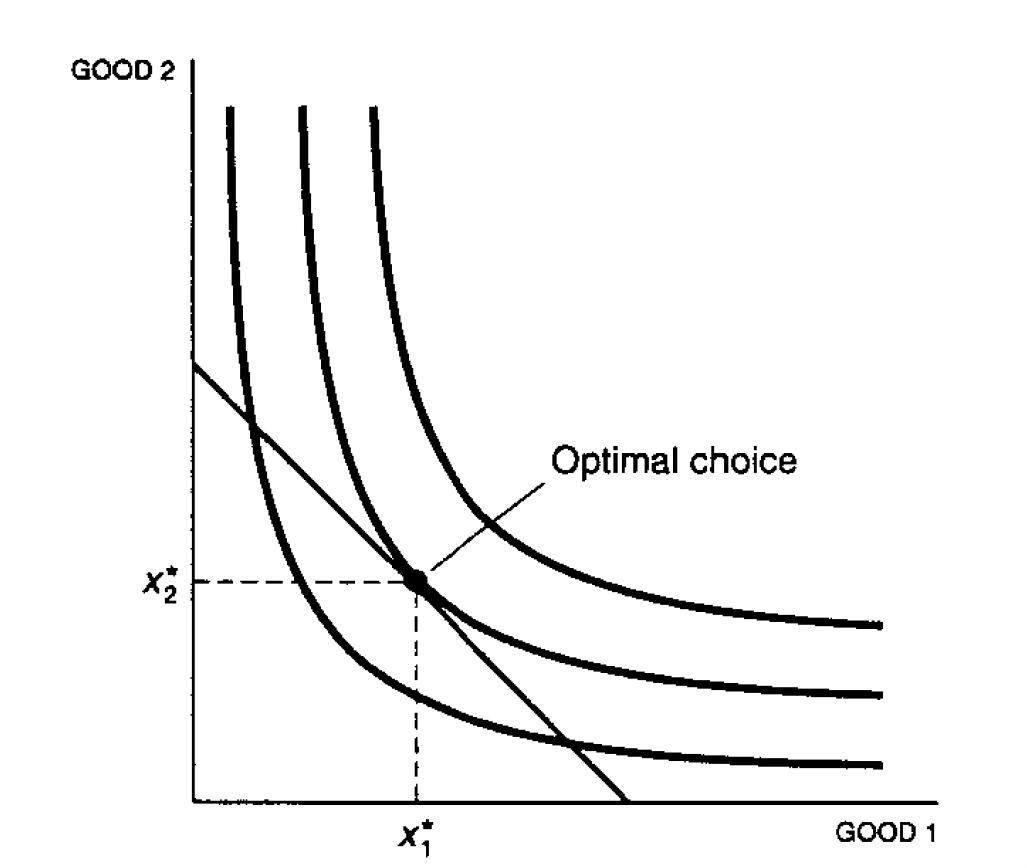
\includegraphics[scale=0.5]{img/fig8-1.png}
    % \caption{Waterloo, ON}
\end{figure}
\begin{itemize}
    \item Budget line: $\{ \mathbf{x} : p_1x_1 + p_2x_2 = m \} \to x_2 = \frac{m}{p_2} - \left( \frac{p_1}{p_2} \right)x_1.$
    \begin{itemize}
        \item Vertical intercept: $\frac{m}{p_2}$
        \item Slope: $-\frac{p_1}{p_2}$
    \end{itemize}
\end{itemize}
The slope of the indifference curve equals the slope of the budget line.  
The optimal consumption bundle happens at the tangent point.

Let $\mathbf{x}^*$ be an optimal choice, and let $\mathbf{dx}$ be a perturbation of $\mathbf{x}^*$ that satisfies the budget constraint. Hence, we must have
\[
    \mathbf{p(x^* \pm dx)} = m.
\]
Since $\mathbf{px} = m$, this equation implies that $\mathbf{p \ dx} = 0$, which in turn implies that $\mathbf{dx}$ must be orthogonal to $\mathbf{p}$.  
For any such perturbation $\mathbf{dx}$, utility cannot change, or else $\mathbf{x}^*$ would not be optimal. 
Hence, we have
\[
\mathbf{D}u(\mathbf{x}^*)\mathbf{dx} = 0.
\]
It in turn implies that:

\begin{enumerate}
    \item $\mathbf{Du}(\mathbf{x}^*)$ must be orthogonal to $\mathbf{dx}$.
    \item $\mathbf{Du}(\mathbf{x}^*)$ must be proportional to $\mathbf{dx}$.
\end{enumerate}

The second derivative of the Lagrangian with respect to goods $i$ and $j$ is $\frac{\partial^2 u(\mathbf{x})}{\partial x_i \partial x_j}$. Hence, the second-order condition can be written as
\[
\mathbf{h}^t \mathbf{D}^2 u(\mathbf{x}^*) \mathbf{h} \leq 0 \quad \forall \ h \ \text{such that} \ \mathbf{ph} = 0.
\]
This condition requires that the Hessian matrix of the utility function is \highlight{negative semidefinite} for all vectors $\mathbf{h}$ orthogonal to the price vector.


\section{Indirect Utility}

\block{Theorem: Indirect Utility Function}{
    Properties of the indirect utility function:
    \begin{enumerate}
        \item $v(\mathbf p, m)$ is nonincreasing in $\mathbf p$; that is, if $\mathbf p^\prime \geq \mathbf p$, $v(\mathbf p^\prime, m) \leq v(\mathbf p, m)$. Similarly, $v(\mathbf p, m)$ is nondecreasing in $m$.
        \item $v(\mathbf p, m)$  is HD-0 in $(\mathbf p, m)$.
        \item $v(\mathbf p, m)$ is a quasi-convex in $\mathbf p$; that is $\{ \mathbf p :v(\mathbf p, m) \leq k \}$ is a convex set for all $k$.
        \item $v(\mathbf p, m)$ is continuous at all $\mathbf p \gg 0, m >0$.
    \end{enumerate}
}

\begin{figure}
    \center
    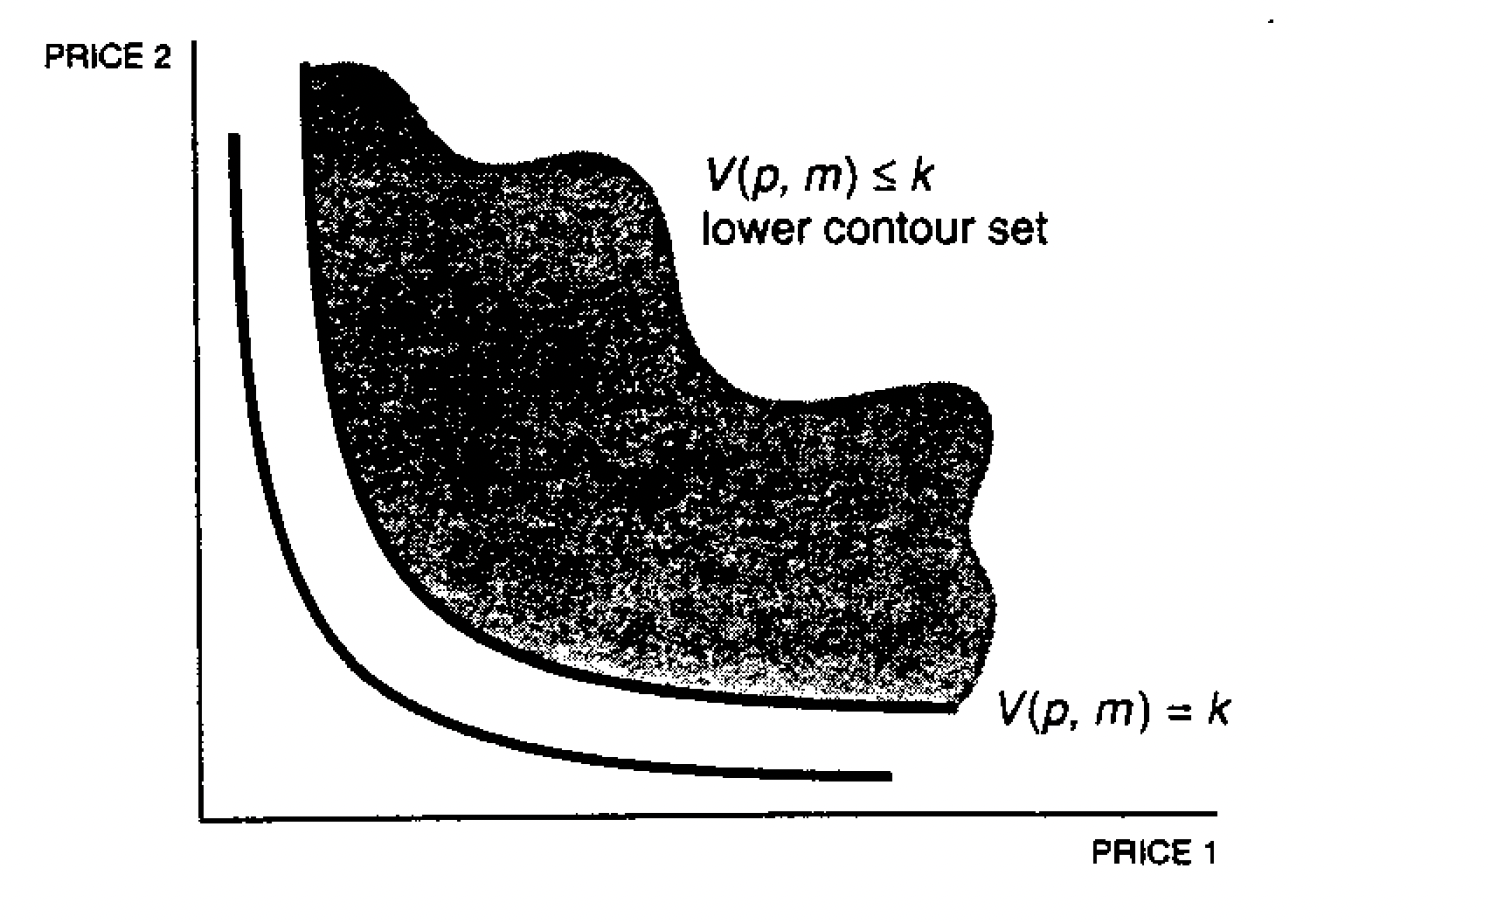
\includegraphics[width=0.7\textwidth]{img/fig7-2}
    \caption{}
\end{figure}

If preference satisfy the local nonsatiation assumption, then $v(\mathbf{p}, m)$ will be strictly increase in $m$. 
Since $v(\mathbf{p}, m)$ is strictly increase in $m$, we can convert the function and solve for $m$ as a function of the level of utility $u$.
That is, given any level of utility, $u$, we can get the minimal amount of income necessay to achieve utility $u$ at price $p$.
The \highlight{inverse of t-}
\highlight{he indirect utility function is known as the \textbf{expenditure function}} and is denoted by $e(\mathbf p, m)$.

\begin{align*}
    e(\mathbf p , u) = \min &\quad \mathbf{px} \\
    \text{s.t.} &\quad u(\mathbf x ) \geq u.
\end{align*}

\block{Definition: Expenditure Function}{
    The expenditure function gives the minimum cost of achieving a fixed level of utility.
}

\begin{figure}
    \center
    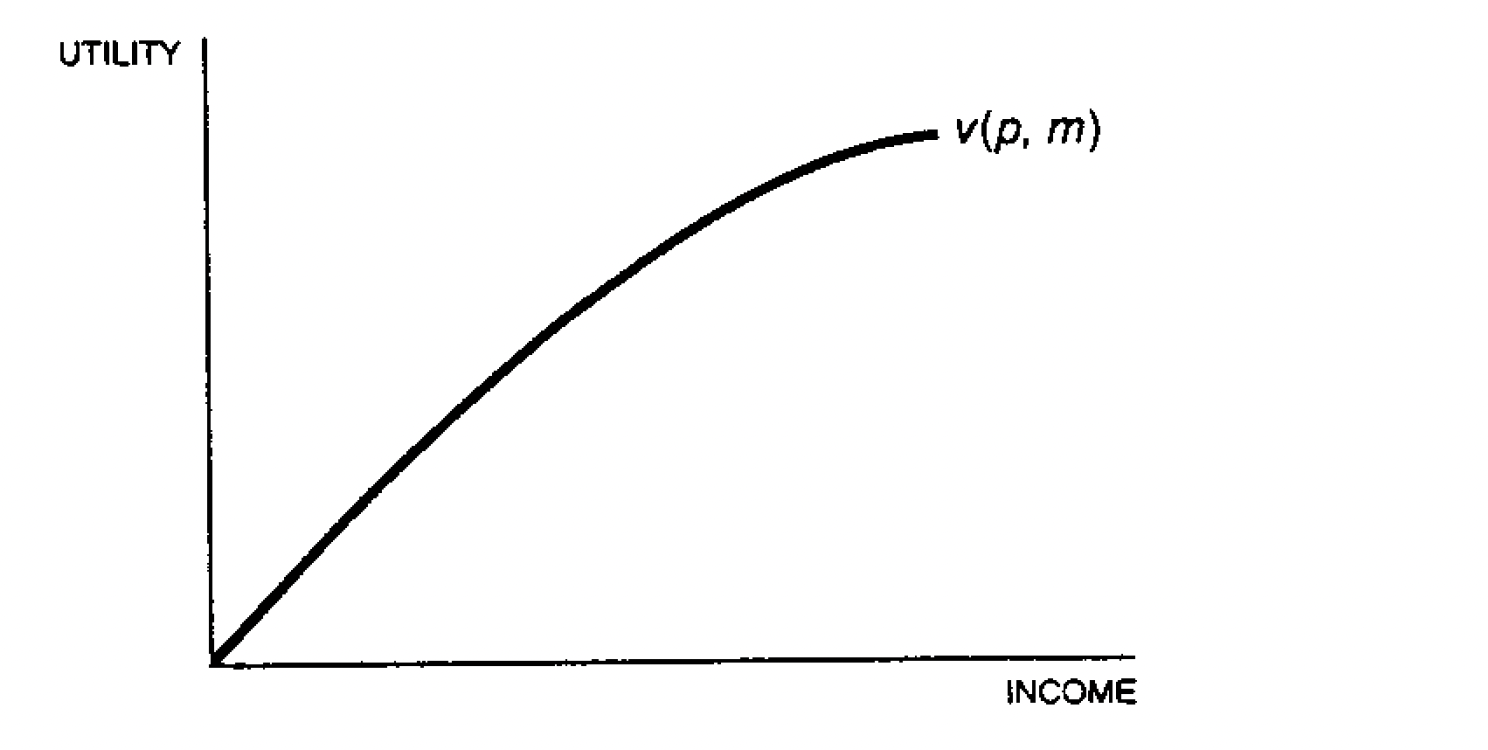
\includegraphics[width=0.7\textwidth]{img/fig7-3}
    \caption{$v^{-1}(\mathbf{p}, m) = e(\mathbf p , u)$}
\end{figure}

\block{Theorem: Expenditure Function}{
    Properties of the expenditure function: (類似 cost function)
    \begin{enumerate}
        \item $e(\mathbf p, u)$ is nondecreasing in $\mathbf p$. %; that is, if $\mathbf p^\prime \geq \mathbf p$, $v(\mathbf p^\prime, m) \leq v(\mathbf p, m)$. Similarly, $v(\mathbf p, m)$ is nondecreasing in $m$.
        \item $e(\mathbf p, u)$ is HD-1 in $\mathbf p$.
        \item $e(\mathbf p, u)$ is a concave in $\mathbf p$. %; that is $\{ \mathbf p :v(\mathbf p, m) \leq k \}$ is a convex set for all $k$.
        \item $e(\mathbf p, u)$ is continuous in $\mathbf p$ at all $\mathbf p \gg 0, m >0$.
        \item If $\mathbf h(\mathbf p, u)$ is the expenditure-minimizing bundle necessary to achieve utility level $u$ at prices $\mathbf p$, then $h_i(\mathbf p, u) = \frac{\partial e(\mathbf{p}, u)}{\partial p_i}$ for $i=1, \dots, k$ assuming the defivative exists and that $p_i > 0$.
    \end{enumerate}
}

\block{Definition: Hicksian Demand Function}{
    The function $h_i(\mathbf p , u)$ is called the Hicksian demand function. 
}
The Hicksian demand function tells us what consumtion bundle achieves a target level of utility and minimizes total expenditure. 
It is sometimes called a compensated demand function as it is constructed by varing prices and income so as to keep the consumer ata fixed level of utility.
Thus, income change are arragned to compensate for the price change.

Hicksian demand are not directly observable since they depend on utility, which is not directly observed.
$\mathbf{x}(\mathbf{p}, m)$ is called uncompensated demand function, Mashallian demand function.


\section{Some Important Identities}

Consider the utility maximization problem and expenditure minimization problem:
\begin{equation*}
    \begin{array}{rl}
        v(\mathbf p, m^*) = \max & \ u(\mathbf{x}) \\
        \text{s.t.} & \ \mathbf{px} \leq m
    \end{array} \iff
    \begin{array}{rl}
        e(\mathbf p, u^*) = \min & \ \mathbf{px} \\
        \text{s.t.} & \ u(\mathbf{x}) \geq u^*.
    \end{array}
\end{equation*}
The answers to these two problems should be the same $\mathbf x^*$.

\block{Theorem}{
    There's some important identities:
    \begin{enumerate}
        \item $e(\mathbf p, v(\mathbf p, m)) \equiv m$. \\
        The minimum expenditure necessary to reach utility $v(\mathbf p, m)$ is $m$. \\
        (在$\mathbf p$的價格下,要達到$v(\mathbf p, m)$效用水準的最小支出為$m$。)
        \item $v(\mathbf p, e(\mathbf p, u)) \equiv u$. \\
        The maximum utility from income $e(\mathbf p, u)$ is $u$. \\
        (在$\mathbf p$的價格及$e(\mathbf p, u)$所得水準之下,可達到的最高效用水準為$u$。)
        \item $x_i(\mathbf p, m)= h_i(\mathbf p, v(\mathbf p, m)).$ \\
        The Marshallian demand at income $m$ is the same as the Hicksian demand at utility $v(\mathbf p, m)$.\\
        (在$\mathbf p$價格、$m$所得水準之下的Marshallian demand等於在$\mathbf p$價格、$v(\mathbf p, m)$效用水準之下的Hicksian demand。)
        \item $h_i(\mathbf p, u) = x_i(\mathbf p, e(\mathbf p, u))$. \\
        The Hicksian demand at utility $u$ is the same as the Marshallian demand at income $e(\mathbf p, u)$.\\
        (在$\mathbf p$價格、$u$效用水準之下的Hicksian demand等於在$\mathbf p$價格、$e(\mathbf p, u)$所得水準之下的Marshallian demand。)
    \end{enumerate}
    $\implies$ Any demanded bundle can be expressed either as the solution to the utility maximization problem or the expenditure minimization problem.
}

\block{Theorem: Roy’s Identities}{
    If $\mathbf x(\mathbf p,m)$ is the Marshallian demand function, then
    \[
        x_i(\mathbf{p}, m) = -\frac{\frac{\partial v (\mathbf{p}, m)}{\partial p_i}}{\frac{\partial v (\mathbf{p}, m)}{\partial m}}
        \quad   \text{for} \ i = 1, \dots, k.
    \]
    \pf{
    Suppose that $\mathbf x^*$ yields a maximal utility of $u^*$ at $(\mathbf p^*, m^*)$. We know from the identities that
    \[
    \mathbf x^* (\mathbf p^*, m^*)
    =
    \mathbf h^* (\mathbf p^*, u^*).
    \]

    From another one of the fundamental identities, we also know that
    \[
        u^* = v(\mathbf p, e(\mathbf p, u^*)).
    \]
    This identity says that no matter what prices are, if you give the consumer the minimal income to get utility $u^*$ at those prices, then the maximal utility he can get is $u^*$.
        
    Since this is an identity we can differentiate it with respect to $p_i$ to get
    \begin{gather*}
        0=
        \frac{\partial v(\mathbf{p^*}, m^*)}{\partial p_i} +
        \frac{\partial v(\mathbf{p^*}, m^*)}{\partial m}
        \frac{\partial e(\mathbf{p^*}, u^*)}{\partial p_i} \\
        \implies
        \mathbf x^* (\mathbf p^*, m^*)
        \equiv
        \mathbf h^* (\mathbf p^*, u^*)
        \equiv
        \frac{\partial e(\mathbf{p^*}, u^*)}{\partial p_i}
        \equiv
        -\frac{\frac{\partial v (\mathbf{p}, m)}{\partial p_i}}{\frac{\partial v (\mathbf{p}, m)}{\partial m}}.
    \end{gather*}
    Since this identity is satisfied for al $(\mathbf p^*, \mathbf m^* )$ and since $\mathbf x^* = \mathbf x(\mathbf p^*, m^*)$, the result is proved.}
}

\block{Theorem: Roy's Identities (Continue)}{
    \pf{
    The utility function is given by
    \[
        v(\textbf p, m) \equiv 
        u(\textbf x (\textbf p, m))
        \quad \dots \ (1)
    \]
        
    If we differentiate this with respect to $p_j$, we find    
    \[
        \frac{\partial v (\mathbf p, m)}{\partial p_j}
        =
        \sum_{i=1}^k
        \frac{\partial u (\mathbf x)}{\partial x_i}
        \frac{\partial x_i}{\partial p_j}
        \quad \dots \ (2)
    \]
        
    Since $\textbf x (\textbf p, m)$ is the demand function, it satisfies the first-order conditions for utility maximization. Substituting the first-order conditions into expression $(2)$ gives
    \[
        \frac{\partial v (\mathbf p, m)}{\partial p_j}
        =
        \sum_{i=1}^k
        \lambda p_i
        \frac{\partial x_i}{\partial p_j}
        \quad \dots \ (3)
    \]
    The demand functions also satisfy the budget constraint $\textbf p\textbf x (\textbf p, m) \equiv m$. Differentiating this identity with respect to $p_j$, we have
    \[
        x_j(\mathbf p, m)+
        \sum_{i=1}^{k}p_i
        \frac{\partial x_i}{\partial p_j}
        =0
        \quad \dots \ (4)
    \]
        
    Substitute $(4)$ into $(3)$ to find
    \[
        \frac{\partial v (\mathbf p, m)}{\partial p_j} = 
        -\lambda x_j(\mathbf p, m)
        \quad \dots \ (5)
    \]
        
    Now we differentiate $(1)$ with respect to $m$ to find
    \[
        \frac{\partial v (\mathbf p, m)}{\partial m}
        =
        \sum_{i=1}^k
        \lambda p_i
        \frac{\partial x_i}{\partial m}
        \quad \dots \ (6)
    \]
        
    Differentiating the budget constraint with respect to $m$, we have    
    \[
        \sum_{i=1}^k
        p_i
        \frac{\partial x_i}{\partial m}
        =1
        \quad \dots \ (7)
    \]
        
    Substituting $(7)$ into $(6)$ gives us    
    \[
        \frac{\partial v (\mathbf p, m)}{\partial m}
        = \lambda
    \]
        
    This equation simply says that the Lagrange multiplier in the first-order condition is the marginal utility of income. Combining $(4)$ and $(7)$ gives us Roy's identity.
    }
}


\section{The Money Metric Utility Function}



\block{Definition: Money Metric Utility Function}{
    How much money would a given consumer need at the prices $\mathbf p$ to be as well off as he could by consuming the bundle $\mathbf x$.
    (在價格$\mathbf p$ 之下,選擇和既有消費組合$\mathbf x$至少一樣好的效用水準的最小支出。)
    \begin{align*}
        \underset{\mathbf{z}}{\min} &\ \mathbf{pz} \\
        \text{s.t.} &\ u(\mathbf{z}) \geq u(\mathbf{x})
    \end{align*}    
    Also known as "minimum income function" or "direct compensation function". 
    An alternative definition is 
    \[
        m(\mathbf{p, x}) \equiv e(\mathbf{p}, u(\mathbf{x})).
    \]
}
\begin{itemize}
    \item If $\mathbf{x}$ is fixed $\to$ $u(\mathbf{x})$ is fixed $\to$ $m(\mathbf{p, x})$ behaves exactly like an expenditure function: \\
    monotonic, homogeneous, concave in $\mathbf p$, and os on.
    \item If $\mathbf{p}$ is fixed $\to$ $m(\mathbf{p, x})$ is an utility function:
\end{itemize}


\block{Definition: Money Metric Indirect Utility Function}{
    \[
        \mu(\mathbf{p}; \mathbf{q}, m) = e(\mathbf{p}, v(\mathbf{q}, m)).
    \]
    $\mu(\mathbf{p}; \mathbf{q}, m)$ measures how much money one would need at prices $\mathbf{p}$ to be as well off as one would be facing prices $\mathbf q$ and having income $m$.
    (在價格$\mathbf{p}$ 之下,支出要達到多少才可以達到 $v(\mathbf q, m)$ 的效用水準。) 
}
$\mu(\mathbf{p}; \mathbf{q}, m)$ behave like an expenditure function with respect to $\mathbf{p}$, but now it behaves like an indirect utility function with respect to $\mathbf q$ and $m$, since it is simply a monotonic transformation of an indirect utility function.
\begin{itemize}
    \item If $v(\mathbf{q}, m)$ is fixed $\to$ $\mu(\mathbf{p}; \mathbf{q}, m)$ is an expenditure function
    \item If $\mathbf{p}$ is fixed $\to$ $\mu(\mathbf{p}; \mathbf{q}, m)$ is an (indirect) utility function
\end{itemize}

\block{Example: Cobb-Douglas utility function}{

}
\block{Example: The CES utility function}{

}

\chapter{Choices}

\section{Comparative statics}

Consumer maximization problem:
\begin{align*}
    \max & \ \text{Utility Function} \\
    \text{s.t.} & \ \text{Budget Constraint} \\
    \implies & \mathbf{x}^*(\mathbf{p}, m) \text{ is the optimal choice.}
\end{align*}

\block{Definition: Income Expension Path}{
Holding price constant and allow income to vary; 
the resulting locus of utility maximizing bundle is known as the \textbf{income expansion path}.
($\mathbf{p}$固定、$m$變動所形成最佳消費組合$\mathbf x$之連線。)
}

\block{Definition: Engle Curve}{
Derive from income expansion curve, it's a function that related to demand for each commodity.
}

\begin{enumerate}
    \item The income expansion path (and thus Engle curve) is a straight line through the origin.
    In this case the consumer is said to have demand curves with unit income elasticity. 
    Such a consumer will consume the same proportion of each commodity at each level of income.
    \begin{itemize}
        \item $\frac{\partial \mathbf{x}}{\partial m} = 0$
    \end{itemize}
    \item The income expansion path bends toward one good or the other, that is as consumer gets more income, he consumes more of both goods but proportionally more of one good (the luxury good) than of the other (the necessary good). 
    (收入增加需求佔比增加為奢侈品;收入增加需求佔比減少為必需品。)
    \begin{itemize}
        \item Luxury good: $\frac{\partial \mathbf{x}}{\partial m} > 1$
        \item Necessary good: $\frac{\partial \mathbf{x}}{\partial m} < 1$
    \end{itemize}
    \item If the income expansion path could bend backwards in this case and increase in income means the consumer actually wants to consume less of one of the good. Such goods are called inferior good;
    goods for which more income means more demand are called normal goods.
    (收入增加需求增加為普通財;收入增加需求減少為劣等財。)
    \begin{itemize}
        \item Normal good: $\frac{\partial \mathbf{x}}{\partial m} > 0$
        \item Inferior good: $\frac{\partial \mathbf{x}}{\partial m} < 0$
    \end{itemize}
\end{enumerate}

\begin{figure}[h]
    \center
    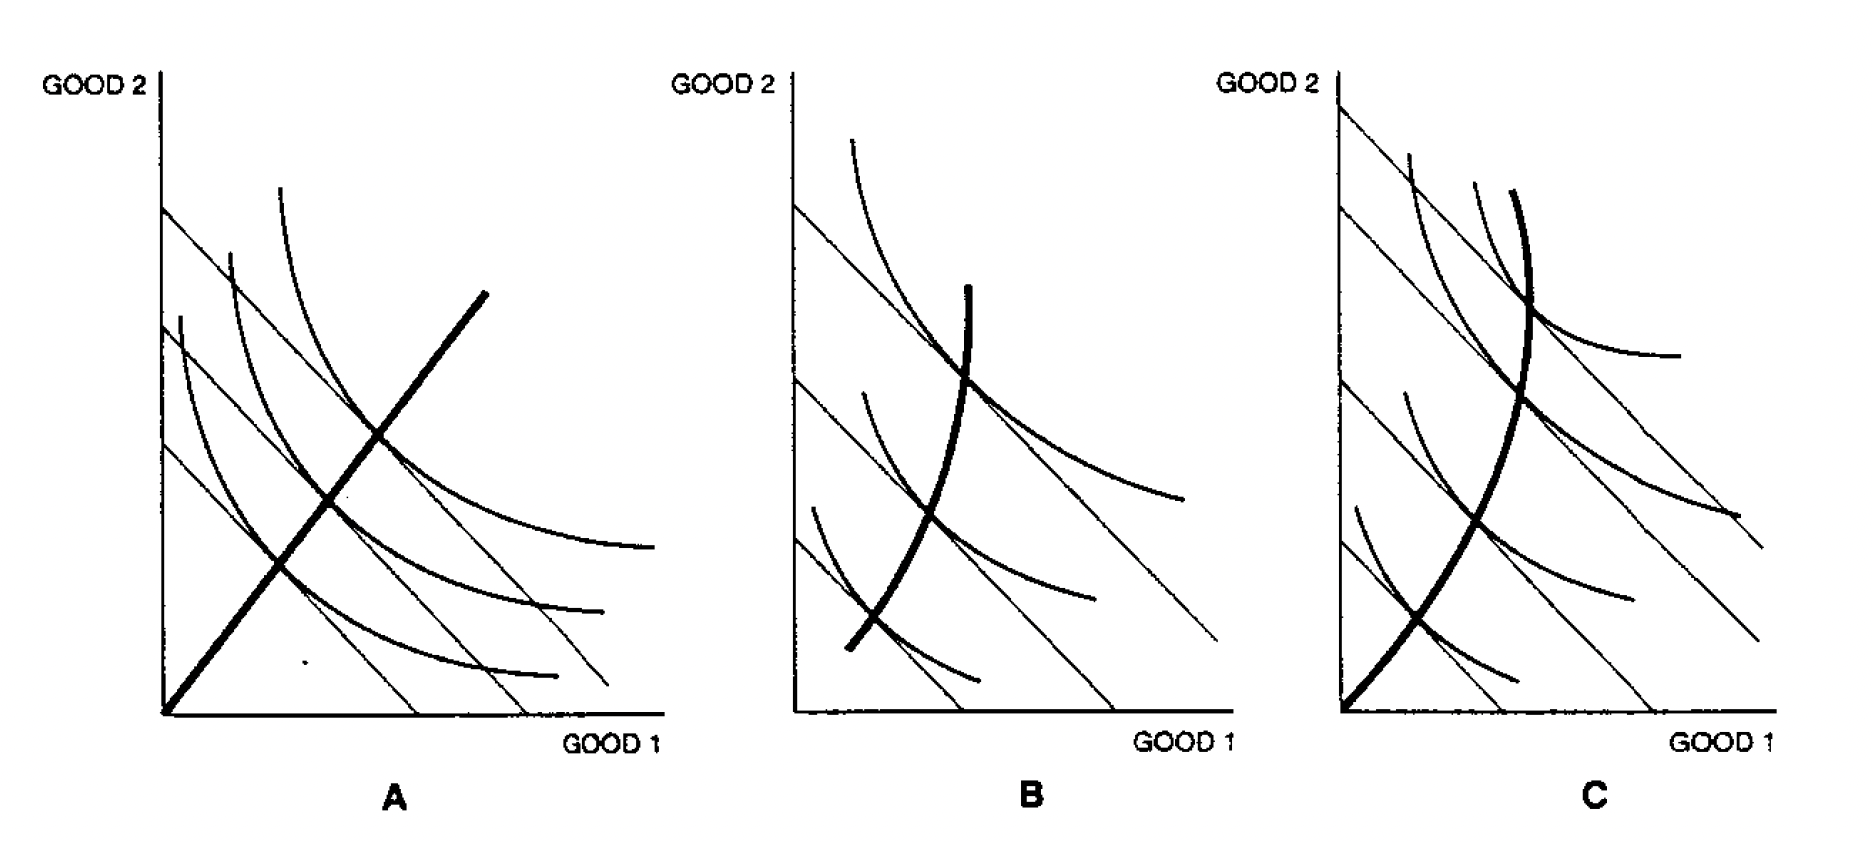
\includegraphics[width=0.7\textwidth]{img/fig8-1-1.png}
    \caption{}
\end{figure}

\block{Definition: Price Offer Curve}{
    Holding income fixed and allow prices to vary. If we let $p_1$ vary and hold $p_2$ and $m$ fixed, our budget line will tilt, and the locus of tangencies will sweep out a curve know as the \textbf{price offer curve}.
    ($m$固定、$\mathbf{p}$變動所形成最佳消費組合$\mathbf x$之連線。)
}

\begin{enumerate}
    \item In ordinary case, lower price for good 1 would lead to greater demand for the good.
    (價格減少需求增加,一般情況。)
    \begin{itemize}
        \item $\frac{\partial \mathbf{x}}{\partial p_i} < 0$
    \end{itemize}
    \item If we have a situation where a decrease in the price of good 1 brings about a decrease demand of good 1.
    Such a good is called \textbf{Giffen good}.
    (價格減少需求減少,季芬財。)
    \begin{itemize}
        \item $\frac{\partial \mathbf{x}}{\partial p_i} > 0$
    \end{itemize}
\end{enumerate}

\begin{figure}[h]
    \center
    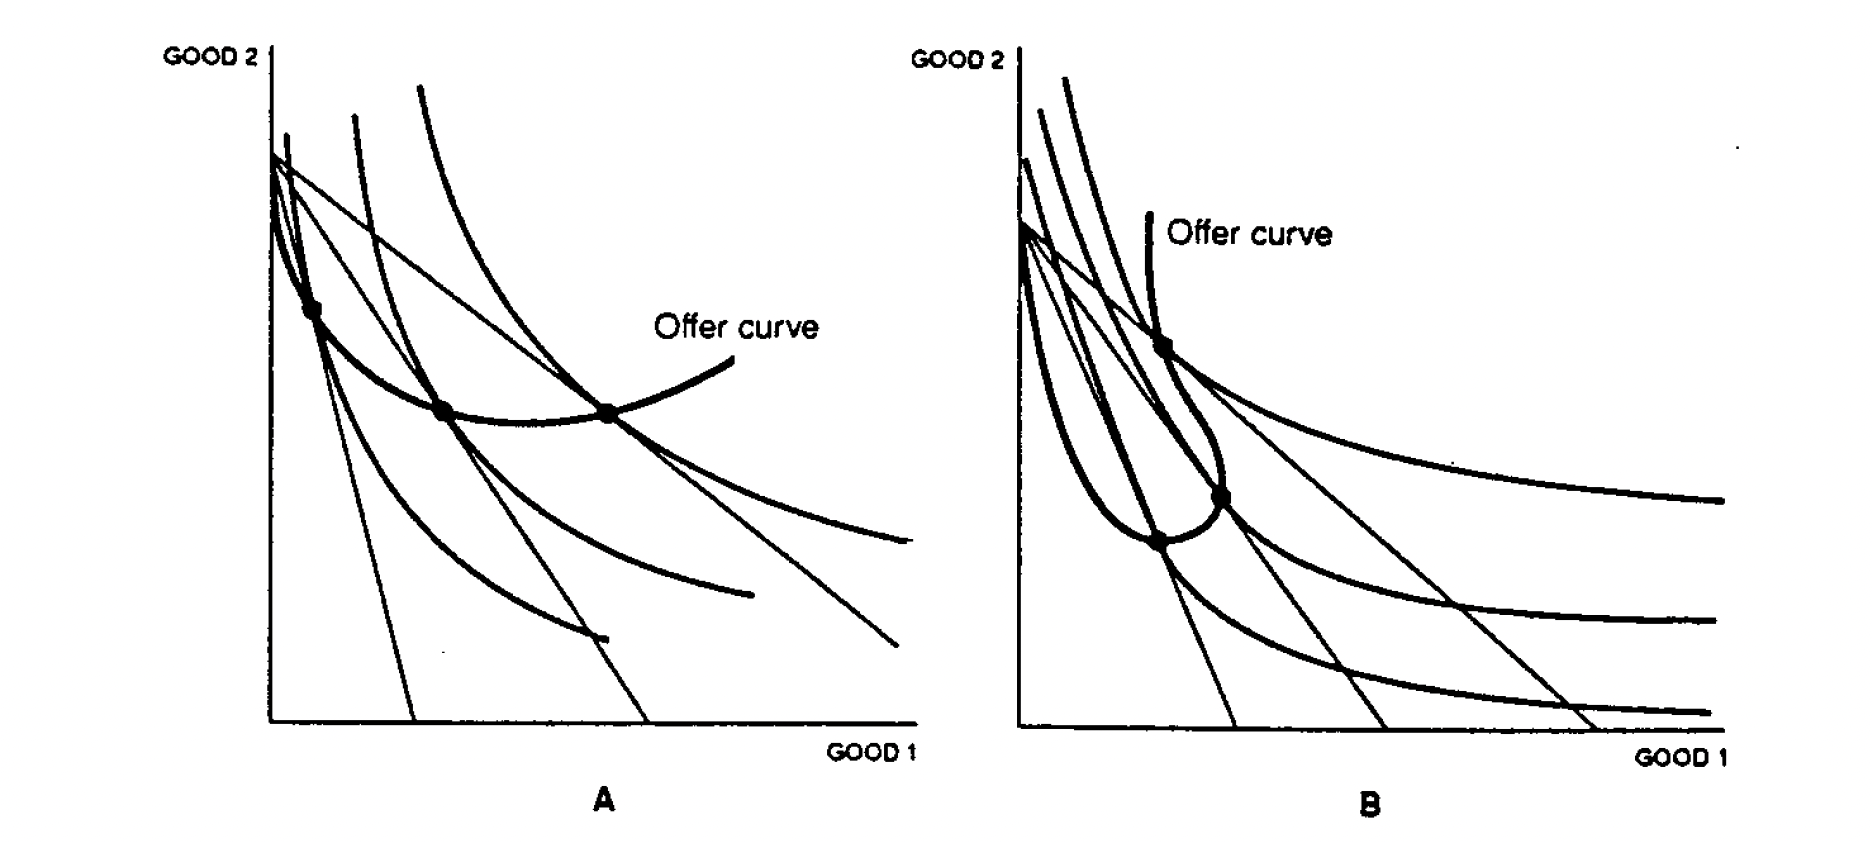
\includegraphics[width=0.7\textwidth]{img/fig8-2.png}
    \caption{}
\end{figure}

\block{Example: Excise and Income Taxes}{
    Initially,  consumers budget constraint is $p_1x_1 + p_2x_2 = m$.
    \begin{enumerate}
        \item \textbf{Excise tax}: \\
        After we impose a tax on sale of good 1 the budget constraint becomes 
        \[
            (p_1+t)x_1 + p_2x_2 = m.
        \]
        Suppose we let after tax level of consumption by $(x_1^*, x_2^*)$, then the revenue collected by the tax is $tx_1^*$.

        \item \textbf{Income tax}: \\
        Suppose now that we decide to collect the same amount of revenue by tax on income. The budget constraint of the consumer would then be 
        \[
            p_1x_1 + p_2x_2 = m-tx_1^*.
        \]
        This is a line with slope $-p_1/p_2$ that through the indifference curve at $(x_1^*, x_2^*)$.
    \end{enumerate}
    Therefore, A consumer is always worse off facing an excise tax than an income tax that generates the same revenue.
}
\begin{figure}[h]
    \center
    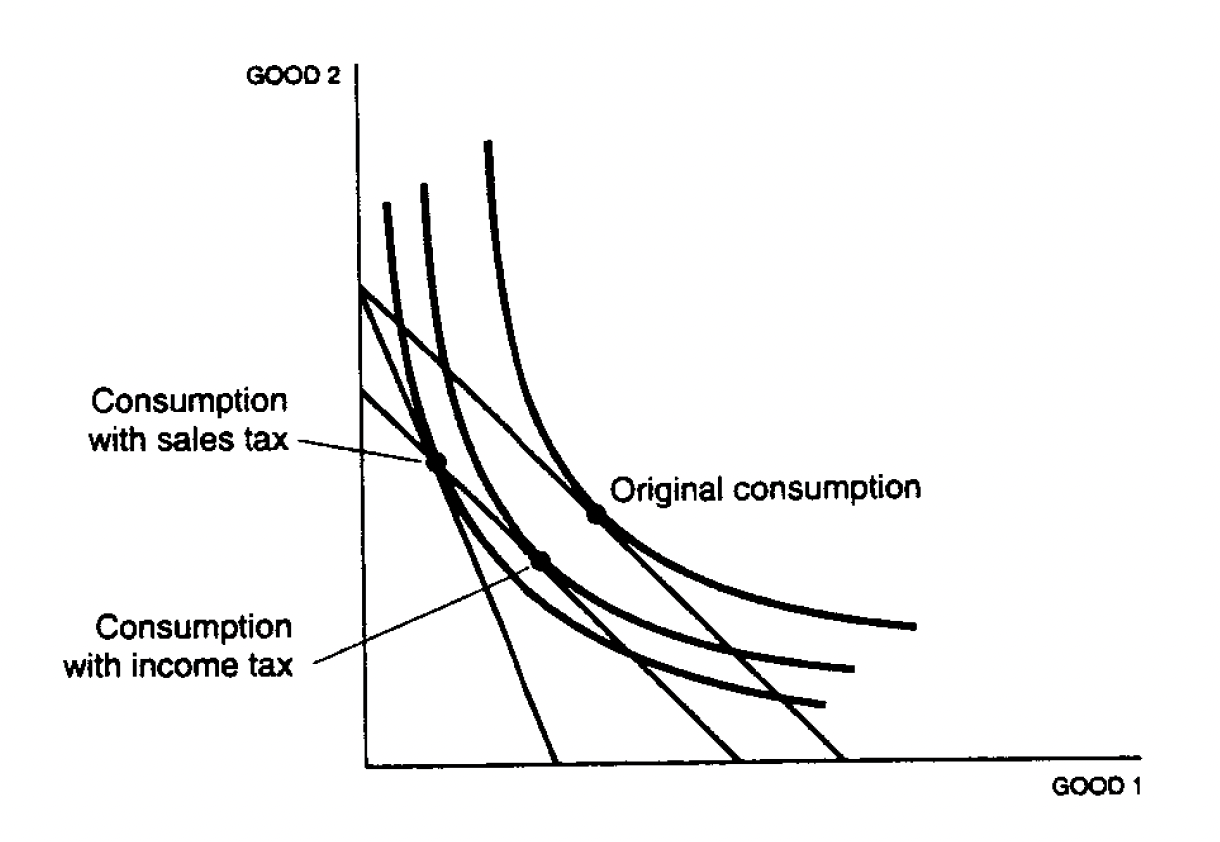
\includegraphics[width=0.7\textwidth]{img/fig8-3.png}
    \caption{}
\end{figure}

\section{The Slusky equation}

The Hicksian, or compensated demand curve, is formally the same as the conditional factor demand. It has all the same properties:
\begin{enumerate}
    \item HD-0
    \item Symmetric, negetive semidefinite  substitution matrix.
\end{enumerate}

\block{Theorem: Slusky equation}{
    \[
        \frac{\partial x_j (\mathbf p, m)}{\partial p_i} = 
        \frac{\partial h_j (\mathbf p, v(\mathbf p, m))}{\partial p_i} -
        \frac{\partial x_j (\mathbf p, m)}{\partial m} x_i (\mathbf p, m)
    \]
    \pf{
        Let $\mathbf x^*$  maximize utility at $(\mathbf p^*,m^*)$ and let  $u^* = u^*(\mathbf x^*)$. It is identically true that 

        \[
        h_j(\mathbf p^*, u^*) \equiv
        x_j(\mathbf p^*, e(\mathbf p^*, u^*)).
        \]

        We can differentiate this with respect to $p_i$ and evaluate the derivative at $\mathrm p^*$ to get 

        \[
        \frac{\partial h_j(\mathbf p^*, u^*) }{\partial p_i} 
        \equiv
        \frac{\partial x_j(\mathbf p^*, m^*) }{\partial p_i} 
        + 
        \frac{\partial x_j(\mathbf p^*, m^*) }{\partial m} \frac{\partial e(\mathbf p^*, u^*) }{\partial p_i}
        \]

        \begin{itemize}
            \item $\frac{\partial h_j(\mathbf p^*, u^*) }{\partial p_i}$ : how the compensated demand changes when $p_i$ changes.
            \item $\frac{\partial x_j(\mathbf p^*, m^*) }{\partial p_i}$ : the change in demand holding expenditure fixed at $m^*$.
            \item $\frac{\partial x_j(\mathbf p^*, m^*) }{\partial m}$ : the change in demand when income changes.
            \item $\frac{\partial e(\mathbf p^*, u^*) }{\partial p_i}$: how much income has to change to keep utility constant, is just $x_i^*$.
        \end{itemize}

        \[
        \implies
        \frac{\partial x_j(\mathbf p^*, m^*) }{\partial p_i} 
        =
        \frac{\partial h_j(\mathbf p^*, u^*) }{\partial p_i} 
        -
        \frac{\partial x_j(\mathbf p^*, m^*) }{\partial m} x_i^*,
        \]

        which is Slutsky equation.
    }
}
The Slutsky equation decomposes the demand change induced by a price change $\Delta p_i$ into two separate effects: the \textbf{substitution effect} and the \textbf{income effect}:
\[
    \Delta x_j \approx
    \frac{\partial x_j(\mathbf p, m) }{\partial p_i} \Delta p_i
    = \underbrace{
    \frac{\partial h_j(\mathbf p, u) }{\partial p_i} \Delta p_i}_{\text{substitution effect}}
    - \underbrace{
    \frac{\partial x_j(\mathbf p, m) }{\partial m} x_i \Delta p_i}_{\text{income effect}}.
\]
General form of Slutsky equation
\begin{align*}
    \mathbf D_p \mathbf x(\mathbf p, m)
    &=
    \mathbf D_p \mathbf h(\mathbf p, u)
    -
    \mathbf D_m \mathbf x(\mathbf p, m) \mathbf x\\
    \begin{bmatrix}
    \frac{\partial x_1(\mathbf p, u) }{\partial p_1} &
    \frac{\partial x_1(\mathbf p, u) }{\partial p_2} \\
    \frac{\partial x_2(\mathbf p, u) }{\partial p_1} &
    \frac{\partial x_2(\mathbf p, u) }{\partial p_2}
    \end{bmatrix}
    &=
    \begin{bmatrix}
    \frac{\partial h_1(\mathbf p, m) }{\partial p_1} &
    \frac{\partial h_1(\mathbf p, m) }{\partial p_2} \\
    \frac{\partial h_2(\mathbf p, m) }{\partial p_1} &
    \frac{\partial h_2(\mathbf p, m) }{\partial p_2}
    \end{bmatrix}
    -
    \begin{bmatrix}
    \frac{\partial x_1(\mathbf p, m) }{\partial m} \\
    \frac{\partial x_2(\mathbf p, m) }{\partial m} 
    \end{bmatrix}
    \begin{bmatrix}
    x_1 & x_2
    \end{bmatrix}
    \\
    &=
    \begin{bmatrix}
    \frac{\partial h_1(\mathbf p, m) }{\partial p_1} &
    \frac{\partial h_1(\mathbf p, m) }{\partial p_2} \\
    \frac{\partial h_2(\mathbf p, m) }{\partial p_1} &
    \frac{\partial h_2(\mathbf p, m) }{\partial p_2}
    \end{bmatrix}
    -
    \begin{bmatrix}
    \frac{\partial x_1(\mathbf p, m) }{\partial m} x_1 &
    \frac{\partial x_1(\mathbf p, m) }{\partial m} x_2\\
    \frac{\partial x_2(\mathbf p, m) }{\partial m} x_1 &
    \frac{\partial x_2(\mathbf p, m) }{\partial m} x_2
    \end{bmatrix}.
\end{align*}
Let $\Delta \mathbf p =(\Delta p_1, \Delta p_2), \ \Delta \mathbf x =(\Delta x_1, \Delta x_2)$,
\begin{align*}
    \begin{bmatrix}
        \Delta x_1 \\ \Delta x_2
    \end{bmatrix}
    &\approx
    \underbrace{
    \begin{bmatrix}
    \frac{\partial h_1}{\partial p_1} &
    \frac{\partial h_1}{\partial p_2} \\
    \frac{\partial h_2}{\partial p_1} &
    \frac{\partial h_2}{\partial p_2}
    \end{bmatrix}
    \begin{bmatrix}
    \Delta p_1 \\ \Delta p_2
    \end{bmatrix}
    }_{\text{substitution effect}}
    - \underbrace{
    \begin{bmatrix}
    \frac{\partial x_1}{\partial m} x_1 &
    \frac{\partial x_1}{\partial m} x_2\\
    \frac{\partial x_2}{\partial m} x_1 &
    \frac{\partial x_2}{\partial m} x_2
    \end{bmatrix}
    \begin{bmatrix}
    \Delta p_1 \\ \Delta p_2
    \end{bmatrix}
    }_{\text{income effect}}
    \\
    &=
    \begin{bmatrix}
    \Delta x_1^s \\ \Delta x_2^s
    \end{bmatrix}
    -
    \begin{bmatrix}
    \Delta x_1^m \\ \Delta x_2^m
    \end{bmatrix}
\end{align*}

\begin{itemize}
    \item Substitution effect: indicate how the Hicksian demand change, it change along indifference curve.
    \item Income effect: indicate the impact of this change on demand, with prices hheld constant at the initial level. (Therefore, the vector lies along the income expansion path.)
\end{itemize}

\begin{figure}[h]
    \center
    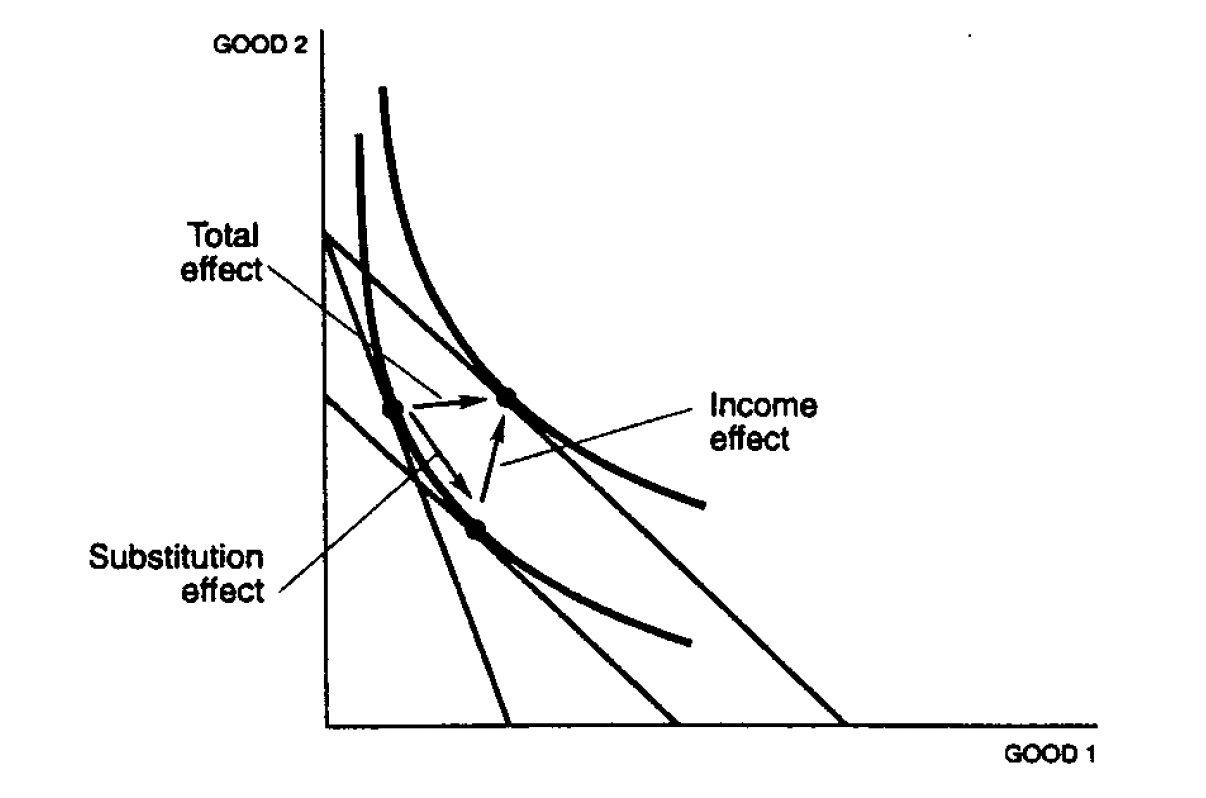
\includegraphics[width=0.7\textwidth]{img/fig8-4.png}
    \caption{}
\end{figure}

\block{Example: The Cobb-Douglas Slutsky Equation}{
    Since $u = x_1^{\alpha-1}x_2^{1-\alpha}$, we have
    \begin{align*}
        v(p_1, p_2, m) &= mp_1^{-a} p_2^{a-1} \\
        e(p_1, p_2, u) &= up_1^{a} p_2^{1-a} \\
        x_1(p_1, p_2, m) &= \frac{am}{p_1} \\
        h_1(p_1, p_2, u) &= \frac{\partial e}{\partial p_1} = ap_1^{a-1} p_2^{1-a} u %\\
        % x_2(p_1, p_2, m) &= \frac{(1-a)m}{p_2} \\
        % h_2(p_1, p_2, u) &= \frac{\partial e}{\partial p_2} = .
    \end{align*}
    Thus, 
    \begin{align*}
        \frac{\partial x_1(\mathbf{p}, m)}{\partial p_1} &= -\frac{am}{p_1^2} \\
        \frac{\partial x_1(\mathbf{p}, m)}{\partial m} &= \frac{a}{p_1} \\
        \frac{\partial h_1(\mathbf p, u)}{\partial p_1} &= a(a-1)p_1^{a-2} p_2^{1-a} u \\
        \frac{\partial h_1(\mathbf p, v(\mathbf p, m))}{\partial p_1} &= a(a-1)p_1^{a-2} p_2^{1-a} (mp_1^{-a} p_2^{a-1}) \\
        &= a(a-1)p_1^{-2}m.
    \end{align*}
    Now plug into the Slutsky equation to find
    \begin{align*}
        \frac{\partial h_1}{\partial p_1}-
        \frac{\partial x_1}{\partial m} x_1 &= 
        \frac{a(a-1)m}{p_1^{-2}} - 
        \frac{a}{p_1}\frac{am}{p_1} \\
        &=\frac{-am}{p_1^2}
        =\frac{\partial x_1}{\partial p_1}
    \end{align*}
}

 
\section{Properties of demand functions}

\block{Theorem: Neoclassical Theory of Consumer Behavior}{
    \begin{enumerate}
        \item (負定) The matrix of substitution terms $\frac{\partial h_j(\mathbf p, u)}{\partial p_i}$ is negative semi-definite because the expenditure function is concave
    
        \[
            \frac{\partial h_j(\mathbf p, u)}{\partial p_i} = 
            \frac{\partial [\frac{\partial e(\mathbf p, u)}{\partial p_j}]}{\partial p_i} = 
            \frac{\partial^2 e(\mathbf p, u)}{\partial p_i \partial p_j}
        \]
        
        \item (對稱) The matrix of substitution terms is symmetric
            
        \[
            \frac{\partial h_j(\mathbf p, u)}{\partial p_i} = 
            \frac{\partial^2 e(\mathbf p, u)}{\partial p_i \partial p_j}= 
            \frac{\partial^2 e(\mathbf p, u)}{\partial p_j \partial p_i}=
            \frac{\partial h_i(\mathbf p, u)}{\partial p_j}
        \]
            
        \item (對角向為負) In particular, “the compensated own-price effect is nonpositive”; that is, the Hicksian demand curve slope downward:
            
            \[
            \frac{\partial h_i(\mathbf p, u)}{\partial p_i} = 
            \frac{\partial^2 e(\mathbf p, u)}{\partial p_i^2} \leq 0
            \]
            
            Since the substitution matrix is negative semi-definite and thus ha non-positive diagonal terms.
            
        \item (替代矩陣負定且對稱) The substitution matrix $(\frac{\partial x_j(\mathbf p, u) }{\partial p_i} + \frac{\partial x_j(\mathbf p, m) }{\partial m} x_i)$ is a symmetric, negative semi-definite matrix.
    \end{enumerate}
}


\section{Comparative statics using the first order condition}

The first order condition of the utility maximization problem gives us:
\begin{align*}
    p_1 x_1(p_1, p_2, m) +p_2 x_2(p_1, p_2, m)-m \equiv 0 \\
    \frac{\partial u( x_1(p_1, p_2, m) , x_2(p_1, p_2, m))}{\partial x_1} -\lambda p_1 \equiv 0 \\
    \frac{\partial u( x_1(p_1, p_2, m) , x_2(p_1, p_2, m))}{\partial x_2} -\lambda p_2 \equiv 0.
\end{align*}

\subsection*{Substitution effect}

Differenting with respect to $p_1$, and arraging in matrix form, we have
\begin{align*}
    \begin{bmatrix}
        0 & -p_1 &-p_2 \\
        -p_1 & u_{11} & u_{12} \\
        -p_2 & u_{21} & u_{22}
    \end{bmatrix}
    \begin{bmatrix}
        \frac{\partial \lambda}{\partial p_1} \\
        \frac{\partial x_1}{\partial p_1}\\
        \frac{\partial x_2}{\partial p_1}
    \end{bmatrix}
    \equiv
    \begin{bmatrix}
        x_1 \\
        \lambda \\
        0
    \end{bmatrix}.
\end{align*}
Using Cramer's rule, 
\[
    \frac{\partial x_1}{\partial p_1} = 
    \frac{
    \begin{vmatrix}
    0 & x_1 &-p_2 \\
    -p_1 & \lambda & u_{12} \\
    -p_2 &0 & u_{22}
    \end{vmatrix}
    }{H}
    =
    \frac{\lambda
    \begin{vmatrix}
    0 & -p_2 \\
    -p_2 & u_{22}
    \end{vmatrix}
    }{H}
    -
    \frac{x_1
    \begin{vmatrix}
    -p_1 & u_{12} \\
    -p_2 & u_{22}
    \end{vmatrix}
    }{H}
\]
\subsection*{Income effect}

Differentiating with respect to $m$.
\[
    \begin{bmatrix}
        0 & -p_1 &-p_2 \\
        -p_1 & u_{11} & u_{12} \\
        -p_2 & u_{21} & u_{22}
        \end{bmatrix}
        \begin{bmatrix}
        \frac{\partial \lambda}{\partial p_1} \\
        \frac{\partial x_1}{\partial p_1}\\
        \frac{\partial x_2}{\partial p_1}
        \end{bmatrix}
        \equiv
        \begin{bmatrix}
        -1 \\
        0 \\
        0
    \end{bmatrix}.
\]
By Cramer's rule,
\[
    \frac{\partial x_1}{\partial m} = 
    \frac{
    \begin{bmatrix}
    0 & -p_1 &-1 \\
    -p_1 & u_{11} & 0 \\
    -p_2 & u_{21} & 0
    \end{bmatrix}
    }{H}
    =
    \frac{
    \begin{vmatrix}
    -p_1 & u_{12} \\
    -p_2 & u_{22}
    \end{vmatrix}
    }{H}.
\] 
\section{The integrability problem}
Skip.

\section{Duality in consumption}
\[
    \begin{array}{r l}
        v(\mathbf{p}) = \max & \ u(\mathbf{x}) \\
        \text{s.t.} & \ \mathbf{px} = 1 
    \end{array}
    \iff
    \begin{array}{r l}
        u(\mathbf{x}) = \min & \ v(\mathbf{p}) \\
        \text{s.t.} & \ \mathbf{px} = 1 
    \end{array}
\]

\block{Example: Solving for the direct utility function}{
    Indirect utility function: $v(p_1, p_2)= -a \ln p_1 -b \ln p_2$.
    The minimization problem:
    \begin{align*}
        \underset{p_1, p_2}{\min} & \ -a \ln p_1 -b \ln p_2 \\
        \text{s.t.} & \ 
        p_1x_1+p_2x_2 = 1 \\
        \implies \mathcal{L} =& -a \ln p_1 -b \ln p_2 - \lambda(p_1x_1+p_2x_2 - 1)
    \end{align*}
    The FOCs are:
    \begin{align*}
        \begin{cases}
            -a /p_1 = \lambda x_1 \\
            -b /p_2 = \lambda x_2 \\
            p_1x_1+p_2x_2 = 1
        \end{cases}
        &\implies
        \begin{cases}
        -a = \lambda x_1 p_1\\
        -b = \lambda x_2 p_2\\
        p_1x_1+p_2x_2 = 1
        \end{cases}
        \\
        &\implies
        \begin{cases}
        -a = \lambda x_1 p_1\\
        -b = \lambda x_2 p_2\\
        (p_1x_1+p_2x_2)\lambda = \lambda
        \end{cases}
        \\
        &\implies -a-b=\lambda
    \end{align*}
    Substitute back to the FOCs to find the inverse demand:
    \[
        \implies
        \begin{cases}
        p_1 = \frac{a}{(a+b)x_1} \\
        p_2 = \frac{b}{(a+b)x_2}
        \end{cases}
    \]
    Substitute the choices of $(p_1, p_2)$ into the indirect utility function:
    \begin{align*}
        u(x_1, x_2)
        =& -a \ln p_1 -b \ln p_2 \\
        =& 
        -a \ln \frac{a}{(a+b)x_1} 
        -b \ln \frac{b}{(a+b)x_2} \\
        =&
        -a(\ln a - \ln(a+b)-\ln x_1)
        -b(\ln b - \ln(a+b)-\ln x_2) \\
        =&
        a \ln x_1 +b \ln x_2
        -a\ln a -b\ln b 
        +(a+b)\ln(a+b) \\
        =&
        a \ln x_1 +b \ln x_2+\text{constant}.
    \end{align*}
    This is Cobb-Douglas utility function.
}

\section{}
Skip
\section{}
Skip


\section{Comparative statics using revealed preference}

\block{Definition: Hicksian Compensation}{
    The demand for the good in question if we change the level of income so as to restore the original level of utility $u$. 
    When $\mathbf p \to \mathbf p + \Delta \mathbf p$,
    \[
        x_i(\mathbf p+ \Delta \mathbf p, m+ \Delta m) \equiv x_i[\mathbf p+ \Delta \mathbf p, e(\mathbf p+ \Delta \mathbf p, u)]
    \]
    (當價格改變,所得要改變多少,使得在新價格之下,可以維持原來的效用水準。需要了解偏好、價格與消費組合。)
}

\block{Definition: Slutsky Compensation}{
    It is the level of demand that arises when income is changed so as to make the original level of consumption possible.
    \begin{align*}
        (\mathbf p+ \Delta \mathbf p) \mathbf{x}( \mathbf p , m) =  m + \Delta m \\
        \implies \Delta \mathbf p \ \mathbf x ( \mathbf{p} , m) = \Delta m
    \end{align*}
    (當價格改變,所得要改變多少,使得在新價格之下,負擔得起原來的消費組合。不需要了解偏好,只要知道價格與消費組合即可。)
}

\begin{figure}[h]
    \center
    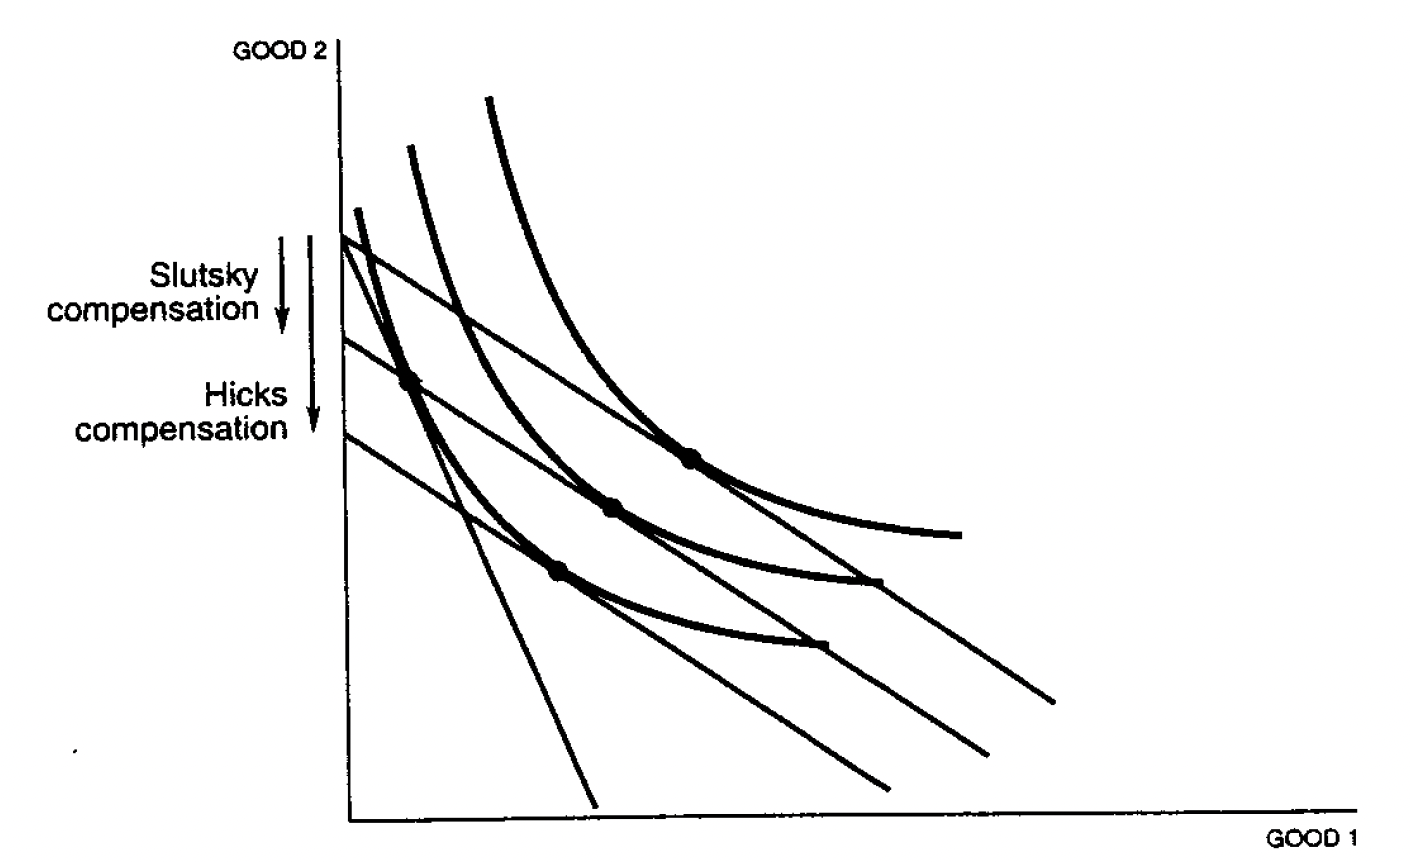
\includegraphics[width=0.7\textwidth]{img/fig8-6.png}
    \caption{}
\end{figure}

\section{}
Skip
\section{}
Skip

\chapter{Demand}

\section{Endowments in the Budget Constraint}

\begin{itemize}
    \item Endowment: $\mathbf{\omega} = (\omega_1, \dots, \omega_k)$
    \item Current market price: $\mathbf{p}$
\end{itemize}

\[
m = \mathbf{p \omega}
\]

The utility maximization problem becomes:
\[
\begin{aligned}
\underset{\mathbf{x}}{\max} &\quad u(\mathbf{x}) \\
\text{s.t.} &\quad \mathbf{p x} = \mathbf{p \omega}.
\end{aligned}
\]

This can be solved using standard techniques to find the demand function $\mathbf{x(p, p \omega)}$:

\[
\begin{aligned}
\frac{dx_i(\mathbf{p, p\omega})}{d p_j} &=
\frac{\partial x_i(\mathbf{p, p\omega})}{\partial p_j}|_{\mathbf{p\omega}=\text{constant}} +
\frac{\partial x_i(\mathbf{p, p\omega})}{\partial m} \omega_j \\
&= \frac{\partial h_i(\mathbf{p}, u)}{\partial p_j} - x_j \frac{\partial x_i(\mathbf{p, p\omega})}{\partial m} + \frac{\partial x_i(\mathbf{p, p\omega})}{\partial m} \omega_j \\
&= \underbrace{\frac{\partial h_i(\mathbf{p}, u)}{\partial p_j}}_{\text{Substitution Effect}} + \underbrace{(\omega_j - x_j) \frac{\partial x_i(\mathbf{p, p\omega})}{\partial m}}_{\text{Income Effect}}.
\end{aligned}
\]

The income effect depends on the net demand for good $j$ rather than the gross demand.

\block{Example: Labor Supply}{
    \begin{enumerate}
        \item Non-labor income: $m$
        \item Consumer chooses two goods:
            \begin{itemize}
                \item Consumption: $c$, price: $p$ (good)
                \item Working hours: $l$, wage: $w$ (bad)
            \end{itemize}
            Utility of consumption: $v(c, l)$. The utility maximization problem is:
            \[
            \begin{aligned}
            \underset{c, l}{\max} &\quad v(c, l) \\
            \text{s.t.} &\quad pc - wl = m.
            \end{aligned}
            \]
        \item Maximum working hours: $\bar{L}$, Leisure: $L = \bar{L} - l$. 
    
        The utility function becomes $u(c, \bar{L} - l) = v(c, l)$, and the problem rewrites as:
    
        \[
        \begin{aligned}
        \underset{c, l}{\max} &\quad u(c, \bar{L} - l) \\
        \text{s.t.} &\quad pc + w(\bar{L} - l) = w \bar{L} + m,
        \end{aligned}
        \]
        or equivalently:
        \[
        \begin{aligned}
        \underset{c, L}{\max} &\quad u(c, L) \\
        \text{s.t.} &\quad pc + wL = w \bar{L} + m.
        \end{aligned}
        \]
    
        Using the Slutsky equation:
        \[
        \frac{dL(p, w, m)}{dw} = \underbrace{-\frac{\partial L(p, w, m)}{\partial w}}_{\text{Substitution Effect}} + \underbrace{\frac{\partial L(p, w, m)}{\partial m}[\bar{L} - L]}_{\text{Income Effect}}.
        \]
    
        An increase in wage can lead to an increase or decrease in labor supply:
        \begin{itemize}
            \item Substitution effect: $\frac{\partial L(p, w, u)}{\partial w}$, higher wages make leisure more expensive (opportunity cost).
            \item Income effect: $\frac{\partial L(p, w, m)}{\partial w}$, higher wages make consumers richer, increasing demand for leisure.
        \end{itemize}
    \end{enumerate}
}


\section{Homothetic Utility Functions}

\block{Recap}{
    \begin{itemize}
        \item A function $f: R^n \to R$ is homogeneous of degree 1 if $f(\mathbf{x}) = t f(\mathbf{x})$ for all $t > 0$.
        \item A function $f(x)$ is homothetic if $f(x) = g(h(x))$, where $g$ is strictly increasing and $h$ is homogeneous of degree 1.
    \end{itemize}
}

Economists often assume utility functions are homogeneous or homothetic since both are defined up to monotonic transformations.
Production function is homogeneous of degree 1 implies 
\begin{itemize}
    \item cost function $c(\mathbf{w}, y) = c(\mathbf{w})y$.
\end{itemize}
\noindent Utility function is homogeneous of degree 1 implies:
\begin{itemize}
    \item expenditure function $e(\mathbf{p}, u) = e(\mathbf{p})u$.
    \item Indirect utility function: $v(\mathbf{p}, m) = v(\mathbf{p})m$.
    \item Demand functions: $x_i(\mathbf{p}, m) = x_i(\mathbf{p})m$ (linear in income).
\end{itemize}


\section{Aggregating Across Goods}

\begin{itemize}
    \item $\mathbf{p}$: price vector of different kinds of meat.
    \item $\mathbf{x}$: consumption vector of different kinds of meat.
    \item $\mathbf{q}$: price vector of other goods.
    \item $\mathbf{z}$: consumption vector of other goods.
\end{itemize}

\[
\begin{aligned}
\underset{\mathbf{x}, \mathbf{z}}{\max} &\quad u(\mathbf{x}, \mathbf{z}) \\
\text{s.t.} &\quad \mathbf{px} + \mathbf{qz} = m.
\end{aligned}
\]

Define price and quantity indices:
\begin{itemize}
    \item Price index: $P = f(\mathbf{p})$
    \item Quantity index: $X = g(\mathbf{x})$
\end{itemize}

\[
\begin{aligned}
\underset{X, \mathbf{z}}{\max} &\quad U(X, \mathbf{z}) \\
\text{s.t.} &\quad PX + \mathbf{qz} = m.
\end{aligned}
\]
The demand function for the quantity index $X$ will be 
\[
    X(P, \textbf q, m) \equiv X(f(\textbf p), \textbf q, m) = g(\textbf x (\textbf p, \textbf q, m)
\]
\subsection*{Hicksian Separability}

Hicksian separability assumes $\mathbf{p} = t \mathbf{p^0}$, leading to:
\[
P = t, \quad X = \mathbf{p^0} \mathbf{x}.
\]
\[
\begin{aligned}
    V(P, \mathbf{q}, m) = 
    \underset{\mathbf{x}, \mathbf{z}}{\max} &\quad u(\mathbf{x}, \mathbf{z}) \\
    \text{s.t.} &\quad P \mathbf{(p^0x)} + \mathbf{qz} = m.
\end{aligned}
\]

By Roy's identity:
\[
X( P, \mathbf{q}, m) = 
- \frac{\partial V(P, \mathbf{q}, m) / \partial P}{\partial V(P, \mathbf{q}, m) / \partial m} 
= \mathbf{p^0} \mathbf{x}(\mathbf p, \mathbf{q}, m).
\]

\block{Example: The two-goods model}{
    $\mathbf{x}$ is a group; $z$ is a single good.

    \[
    \begin{aligned}
    \underset{\mathbf{x}, z}{\max} &\quad u(\mathbf{x}, z) \\
    \text{s.t.} &\quad \mathbf{px} + qz = m.
    \end{aligned}
    \]

    \[
    \mathbf{p} = P\mathbf{p^0}.
    \]
    Since the demand function is homogeneous in degree zero
    \[
    \mathbf{z} = \mathbf{z}(P, \mathbf{q}, m) = 
    \mathbf{z}\left(\frac{\mathbf{q}}{P}, \frac{m}{P}\right).
    \]
    This says that the demand for the $z$-good depends on the relative price of the $z$-good to all other goods and income, devided by the prices of "all other goods".

    In practice, the price index for all other goods is usually taken to be some standard consumer price index. The demand for the $z$-good becomes a function of only two variables:
    \begin{enumerate}
        \item The price of the $z$-good relative to the CPI.
        \item Income relative to the CPI.
    \end{enumerate}
}

\subsection*{Functional Separability}

Let us suppose that the underlying preference order has the property that 
\[ 
(\mathbf x, \mathbf z) \succ (\mathbf x^\prime, \mathbf z) \iff (\mathbf x, \mathbf z^\prime) \succ (\mathbf x^\prime, \mathbf z^\prime)
\]
for all consumption bundles \(\mathbf x, \mathbf x^\prime,\mathbf z, \mathbf z^\prime\). 
This says that the preferences over the \(\mathbf x\)-goods are independent of the \(\mathbf z\)-goods.
\highlight{(不管消費組合\(\mathbf z\)為何,\(\mathbf x \succ \mathbf x^\prime\),永遠偏好\(\mathbf x \)消費組合。)}

If 
\begin{enumerate}
    \item The independence property is satisfied
    \item The preference are locally nonsatiated
\end{enumerate}
Then 
\[
u (\mathbf x, \mathbf z ) = U(v(\mathbf x ), \mathbf z),
\] where 
\begin{enumerate}
    \item \( U(v, \mathbf z) \) is an increse function of \( v \).
    \item \( v(\mathbf x) \) is subutility of \( \mathbf x\).
    \item \( \mathbf z \) is the level of consumption of the \(\mathbf z\)-goods.
\end{enumerate}
We say that the utility function is \highlight{weekly separable}. (具弱可分性。)

Let \(m_x = \mathbf{px}(\mathbf{p, q, }m) \) be the optimal expenditure on the \( \mathbf x \)-goods. 
If the overall utility function is weakly separable, the optimal choice of the \( \mathbf x \)-goods can be found by solving the following subutility maximization problem:
\begin{align*}
    \underset{}{\max} &\quad v(\mathbf{x}) \\
    \text{s.t.} &\quad \mathbf{px} = m_x.
\end{align*}
This means that the demand for the \( \mathbf x \)-goods is only a function of the prices of the \( \mathbf x \)-goods and the expenditure on the  \( \mathbf x \)-goods, \( m_x \).
The prices of the other goods only relevant insofar as they determine the expenditure on the \( \mathbf x \)-goods. 

The demand for the \( \mathbf x \)-goods, \( \mathbf x (\mathbf p, m_x) \) are conditional demand functions since they give demand for the \( \mathbf x \)-goods conditional on the level of expenditure on these goods.
(例:牛肉的需求可以看作牛、羊、豬、雞價格與總消費的函數。)

Let \( e (\mathbf p , v) \) be the expenditure function for the subutility maximization problem. 
We can rewrite the overall maximization problem of the consumer as 
\begin{align*}
    \underset{v, \mathbf{z}}{\max} &\quad U(v, \mathbf{z}) \\
    \text{s.t.} &\quad e (\mathbf p , v) + \mathbf{qz} = m.
\end{align*}
This is almost in the form we want:
\begin{enumerate}
    \item \( X = v(\mathbf x) \) is a suitable quantity index for the \( \mathbf x \)-goods.
    \item \( P = e(\mathbf p, v) \) is a nonlinear function of \( \mathbf p \) and \( X = v \), which isn't what we want. 
\end{enumerate}

In order to have a budget constraint that is linear in quantity index, we need to assume that the subutility function has a special structure -- assume the subutility function is homothetic.
Then we can write 
\begin{itemize}
    \item Expenditure Function: \( e(\mathbf p, v) = e(\mathbf p) v \)
    \item Quantity Index: \( X = v(\mathbf x) \)
    \item Price Index: \( P = e( \mathbf p ) \)
    \item Utility Function: \( U(X, \mathbf z)\)
\end{itemize}
We ge the same \( X \) if we solve 
\begin{align*}
    \underset{X, \mathbf{z}}{\max} &\quad U(X, \mathbf{z}) \\
    \text{s.t.} &\quad PX+ \mathbf{qz} = m
\end{align*}
as if we solve 
\begin{align*}
    \underset{\mathbf{x, z}}{\max} &\quad u(v(\mathbf{x}), \mathbf{z}) \\
    \text{s.t.} &\quad \mathbf{px} + \mathbf{qz} = m
\end{align*}
and then aggregate using \( X = v(\mathbf x) \).

In this formulation we can think of the consumption decision as taking place in two stages:
\begin{enumerate}
    \item The consumer considers how much of the composite commodity (e.g., meat) to consume as a function of a price index.
    \item Then the consumer considers how much beef to consume given the prices of the various sorts of meat and the total expenditure on meat, which is the solution to the subutility maximization problem.
\end{enumerate}


\section{Aggregating Across Consumers}

Continuity of individual demand functions is a \highlight{sufficient but not necessary condition} for continuity of aggregate demand funtion. 
At any price greater than \( r_i \), consumer \( i \) demands zero of the good.
If the price is less than or equal to \( r_i \), consumer \( i \) will demand one unit of the good. 
The price \( r_i \) is called the \( i \)-th consumer's \highlight{reservation price}. 

The aggregate demand for washing machines is given by 
\[
    X(p) = \text{number of consumers whose reservation price is at least $p$}
\]
If there are a lot of consumers with dispersed reservation price, it would make sense to think of this as a continuous function.
The aggregate demand function will in general possess no interesting properties other than \highlight{homogeneity and continuity}.

Suppose an individual consumers' indirect utility functions take the \textbf{Gorman form}:
\[
    v_i(\mathbf p, m_i) = a_i(\mathbf{p}) + b(\mathbf{p}) m_i
\]
where 
\begin{itemize}
    \item \( a_i(\mathbf{p}) \) can differ from consumer to consumer
    \item \( b(\mathbf{p}) \) is assume to be identical for all consumers.
\end{itemize}
By Roy's identity, the demand for good \( j \) of consumer \( i \) will take the form:
\begin{align*}
    x_i^j(\mathbf{p}, m_i) &= -\frac{ \partial v_i / \partial p_j}{ \partial v_i / \partial m} \\
    &= -\frac{
        \frac{\partial a_i(\mathbf{p})}{ \partial p_j } + \frac{ \partial b }{ \partial p_j} m_i
    }{b(\mathbf{p})} \\
    &= -\frac{ \frac{\partial a_i(\mathbf{p})}{ \partial p_j } }{ b(\mathbf{p}) } - \frac{ \frac{b(\mathbf{p})}{ \partial p_j } }{ b(\mathbf{p}) } m_i \\
    &= \alpha_i^j(\mathbf{p}) - \beta^j(\mathbf{p}) \cdot m_i \\
    \implies \frac{ \partial x_i^j(\mathbf{p}, m_i) }{ \partial m_i } &= \beta^j(\mathbf{p})
\end{align*}
The marginal propensity to consume good \( j \), \( \frac{ \partial x_i^j(\mathbf{p}, m_i) }{ \partial m_i } \), is \highlight{independent of the level of income}
\highlight{of any consumer and also constant across consumers since \( b(\mathbf{p}) \) is constant across consumers.} 

The aggregate demand for good \( j \) will take the form 
\[
    X^j( \mathbf{p}, m_1, \cdots, m_n) = -\left[ \sum_{i=1}^{n} \frac{ \frac{\partial a_i(\mathbf{p})}{ \partial p_j } }{ b(\mathbf{p}) } + \frac{ \frac{b(\mathbf{p})}{ \partial p_j } }{ b(\mathbf{p}) } \sum_{i=1}^{n} m_i \right].
\]
This demand function can be generated by a representative consumer. 
His (or her) representative indirect utility function is given by
\begin{align*}
    V(\mathbf p, M) &= \sum_{i=1}^{n} \left( a_i(\mathbf{p}) + b(\mathbf{p}) m_i \right)  \\
    &= A(\mathbf p) + B(\mathbf p) M
\end{align*}
where \( M = \sum_{i=1}^{n} m_i \). It show that the \highlight{Gorman form is not only sufficient} for the representative consumer model to hold, \highlight{but it is also necessary}. (只要消費者的間接效用函數可寫成 Gorman form,可用代表性消費分析,方便我們分析。)

\block{Example}{
    Suppose that there are only two consumers. Then the aggregate demand for good \( j \) can be writen as 
    \begin{align*}
        X^j( \mathbf{p}, m_1, m_2) &= x_1^j(\mathbf p, m_1) + x_2^j(\mathbf p, m_2) \\
        \implies \frac{\partial X^j( \mathbf{p}, M)}{ \partial M } &\equiv \frac{ \partial x_1^j(\mathbf p, m_1) }{ \partial m_1 } \equiv \frac{ \partial x_2^j(\mathbf p, m_2) }{ \partial m_2 }.
    \end{align*}
    Hence, marginal propensity to consume good \( j \) must be the same for all consumers.
    \[
        \frac{\partial^2 X^j( \mathbf{p}, M)}{ \partial M^2 } \equiv \frac{ \partial^2 x_1^j(\mathbf p, m_1) }{ \partial m_1^2 }  \equiv \frac{ \partial^2 x_2^j(\mathbf p, m_2) }{ \partial m_2^2 }  = 0
    \]
    Consumer 1's demand for good \( j \) and consumer 2's demand for good \( j \) are affine (仿射) in income.
    Therefore, the demand function for good \( j \) take the form 
    \[
        x_i^j(\mathbf{p}, m_i) = \alpha_i^j(\mathbf{p}) - \beta^j(\mathbf{p}) \cdot m_i.
    \]
    If this is true for all goods, the indirect utility funciton for each consumers must have the Gorman form.
    \highlight{(若對所有產品皆符合,則消費者之間接效用函數一定是 Gorman fo-}
    \highlight{rm。)}
}

\noindent Two special cases of utility funcitons having a Gorman form:
\begin{enumerate}
    \item Homothetic utility function: \( V( \mathbf p, m) = V( \mathbf p) \cdot m\)
    \item Quasi-linear utility function: \( V( \mathbf p, m) = V( \mathbf p) + m\)
\end{enumerate}
Many of the properties possessed by homothetic and/or quasi-linear utility are also possessed by Gorman form.


\section{Inverse demand functions}

Since demand functions are HD-0, we can fixed income at \(m = 1\).
\begin{align*}
    \underset{}{\max} &\quad u \\
    \text{s.t.} &\quad \mathbf{px} = 1 \\
    \implies & \mathcal{L} = u-\lambda(\mathbf{px} -  1) \\
    \implies & \frac{\partial \mathcal{L}}{\partial x_i} = \frac{\partial u}{\partial x_i} - \lambda p_i = 0 \implies p_i = \frac{1}{\lambda} \frac{\partial u}{\partial x_i} \\
    \implies & \mathbf{px} = \sum_{i=1}^{k} p_i x_i = \sum_{i-1}^{k} \left( \frac{1}{\lambda} \frac{\partial u}{\partial x_i} \right) x_i = \frac{1}{\lambda} \sum_{i=1}^{k} \left( \frac{\partial u}{\partial x_i} \right) x_i = 1 \\
    \implies & \sum_{i=1}^{k} \left( \frac{\partial u}{\partial x_i} \right) x_i = \lambda \\
    \implies & p_i(\mathbf x) = \frac{1}{\lambda} \frac{\partial u(\mathbf x)}{\partial x_i} = \frac{\frac{\partial u(\mathbf x)}{\partial x_i}}{\sum_{j=1}^{k} \left( \frac{\partial u(\mathbf x)}{\partial x_j} \right) x_j} 
\end{align*}
This is the indirect (inverse) demand function as function of \( \mathbf x \). 
If the utility is quasi-concave so that these necessary conditions are indeed sufficient for maximization, then this will give us the inverse demand relationship.

There is a dual version of the above formula for inverse demands. Since xxxx, to simplify without lose of the generosity, we can fixed income at \(m = 1\).
\begin{align*}
    u(\mathbf x) = \underset{}{\min} &\quad \mathbf v(\mathbf p) \\
    \text{s.t.} &\quad \mathbf{px} = 1 \\
    \implies & \mathcal{L} = v-\mu(\mathbf{px} -  1) \\
    \implies & \frac{\partial \mathcal{L}}{\partial p_i} = \frac{\partial v}{\partial p_i} - \mu x_i = 0 \implies \mu x_i p_i = \frac{\partial v}{\partial p_i} p_i  \\
    \implies & \mathbf{px} = \sum_{i=1}^{k} p_i x_i = \sum_{i-1}^{k} \left( \frac{1}{\mu} \frac{\partial v}{\partial p_i} \right) p_i = \frac{1}{\mu} \sum_{i=1}^{k} \left( \frac{\partial v}{\partial p_i} \right) p_i = 1 \\
    \implies & \sum_{i=1}^{k} \left( \frac{\partial v}{\partial p_i} \right) p_i = \mu \\
    \implies & x_i(\mathbf p) = \frac{1}{\mu} \frac{\partial v(\mathbf p)}{\partial p_i} = \frac{\frac{\partial v(\mathbf p)}{\partial p_i}}{\sum_{j=1}^{k} \left( \frac{\partial v(\mathbf p)}{\partial p_j} \right) p_j} 
\end{align*}
This is the direct demand funciton as function of \( \mathbf p \). The both functions have the same form.

\section{Continuity of demand functions}

Skip.

\chapter{consumer's Surplus}

\section{Compensating and Equivalent Variations}

\begin{itemize}
\item $(\mathbf{p}^0, m^0)$: status quo
\item $(\mathbf{p}^\prime, m^\prime)$: proposed change
\end{itemize}
Measure of the welfare change involved in moving from $(\mathbf{p}^0, m^0)$ to $(\mathbf{p}^\prime, m^\prime)$ is just the difference in indirect utility:
\[
    v(\mathbf{p}^\prime, m^\prime)-v(\mathbf{p}^0, m^0).
\]
We can adopt the indirect money metric utility function
\[
    \mu(\mathbf{q}; \mathbf{p}, m) = e(\mathbf{q}, v(\mathbf{p}, m))
\]
The above utility becomes
\[
    \mu(\mathbf{q}; \mathbf{p}^\prime, m^\prime)-
    \mu(\mathbf{q}; \mathbf{p}^0, m^0)
\]
\block{Compensating and Equivalent Variations}{
    \begin{align*}
        EV &= \mu( \mathbf{p}^0; \mathbf{p}^\prime, m^\prime)
        - \mu( \mathbf{p}^0; \mathbf{p}^0, m^0)
        = \mu( \mathbf{p}^0; \mathbf{p}^\prime, m^\prime) - m^0
    \end{align*}
    \begin{itemize}
        \item Equivalent variation: It uses the current prices as the base and asks what income change at the current prices would be equivalent to the proposed change in terms of its impact on utility.
    \end{itemize}
    \begin{align*}
        CV &= \mu( \mathbf{p}^\prime; \mathbf{p}^\prime, m^\prime)
        - \mu( \mathbf{p}^\prime; \mathbf{p}^0, m^0)
        = m^\prime - \mu( \mathbf{p}^\prime; \mathbf{p}^0, m^0)
    \end{align*}
    \begin{itemize}
        \item Compensating variation: It uses the new prices as the base and asks what income change would be necessary to compensate the consumer for the price change.
    \end{itemize}
}
Both of these numbers are reasonable measures of the welfare effect of a price change. Their magnitudes will generally differ because the value of a dollar will depend on what th relevant price are. However, their sign will always be the same since they both measure the same utility differences, just using a different utility function.

If you are trying to arrange for some compensation scheme at the new prices, then the compensating variation seems reasonable. However, if you are simply trying to get a reasonable measure of "willingness to pay," the equivalent variation is probably better. This is so for two reasons:
\begin{enumerate}
    \item The equivalent variation measures the income change at current prices, and it is much easier for decision makers to judge the value of a dollar at current prices than at some hypothetical prices.
    \item Second, if we are comparing more than one proposed policy change, the compensating variation uses different base prices for each new policy while the equivalent variation keeps the base prices fixed at the status quo.
\end{enumerate}
Thus, the equivalent variation is more suitable for comparisons among a variety of projects.

In summary, the compensating and equivalent variations are in fact observable if the demand functions are observable and if the demand functions satisfy the conditions implied by utility maximization.

\section{Consumer Surplus}

\block{Consumer Surplus}{
    If $x(p)$ is the demand for some good as a function of its price, then the consumer's surplus associated with a price movement from $p^0$ to $p^\prime$ is
    \[
        CS=\int_{p^0}^{p^\prime} x(t) dt.
    \]
}
It turns out that when the consumer's preferences can be represented by a quasilinear utility function, consumer's surplus is an exact measure of welfare change. More precisely, when utility is quasilinear, the compensating variation equals the equivalent variation, and both are equal to the consumer's surplus integral. For more general forms of the utility function, the compensating variation will be different from the equivalent variation and consumer's surplus will not be an exact measure of welfare change.

\section{Quasilinear utility}
Suppose that there exists a monotonic transformation of utility that has the form
\[
    U(x_0,x_1, \dots, x_k) = x_0 + U(x_1, \dots, x_k).
\]
Note that the utility function is linear in one of the goods, but (possibly) nonlinear in the other goods. For this reason we call this a quasilinear utility function.

\subsection{Two goods case}
\begin{align*}
    \underset{x_0, x_1}{\max} & \ x_0 + u(x_1) \\
    \text{s.t.} & \ x_0 + p_1x_1 = m \\
    \implies \underset{x_1}{\max} & \ (m-p_1x_1) + u(x_1)
\end{align*}
Take the FOC, we get inverse demand function,
\[
    u^\prime(x_1) = p_1
\]

\chapter{Examples} 

\section{Theorem System}

\defn{Definition Name}{
    A defintion.
}

\thmr{Theorem Name}{mybigthm}{
    A theorem.
}

\lem{Lemma Name}{
    A lemma.
}

\fact{
    A fact.
}

\cor{
    A corollary.
}

\prop{
    A proposition.
}

\clmp{}{
    A claim.
}{
    A reference to Theorem~\ref{thm:mybigthm}
}

\pf{
    Veniam velit incididunt deserunt est proident consectetur non velit ipsum voluptate nulla quis. Ea ullamco consequat non ad amet cupidatat cupidatat aliquip tempor sint ea nisi elit dolore dolore. 

    Laboris labore magna dolore eiusmod ea ex et eiusmod laboris. Et aliquip cupidatat reprehenderit id officia pariatur. 
}

\ex{
    Nostrud esse occaecat Lorem dolore laborum exercitation adipisicing eu sint sunt et. Excepteur voluptate consectetur qui ex amet esse sunt ut nostrud qui proident non. Ipsum nostrud ut elit dolor. Incididunt voluptate esse et est labore cillum proident duis.
}

\rmk{
    Some remark.
}

\rmkb{
    Some more remark.
}

\section{Pictures}

\begin{figure}[H]
    \center
    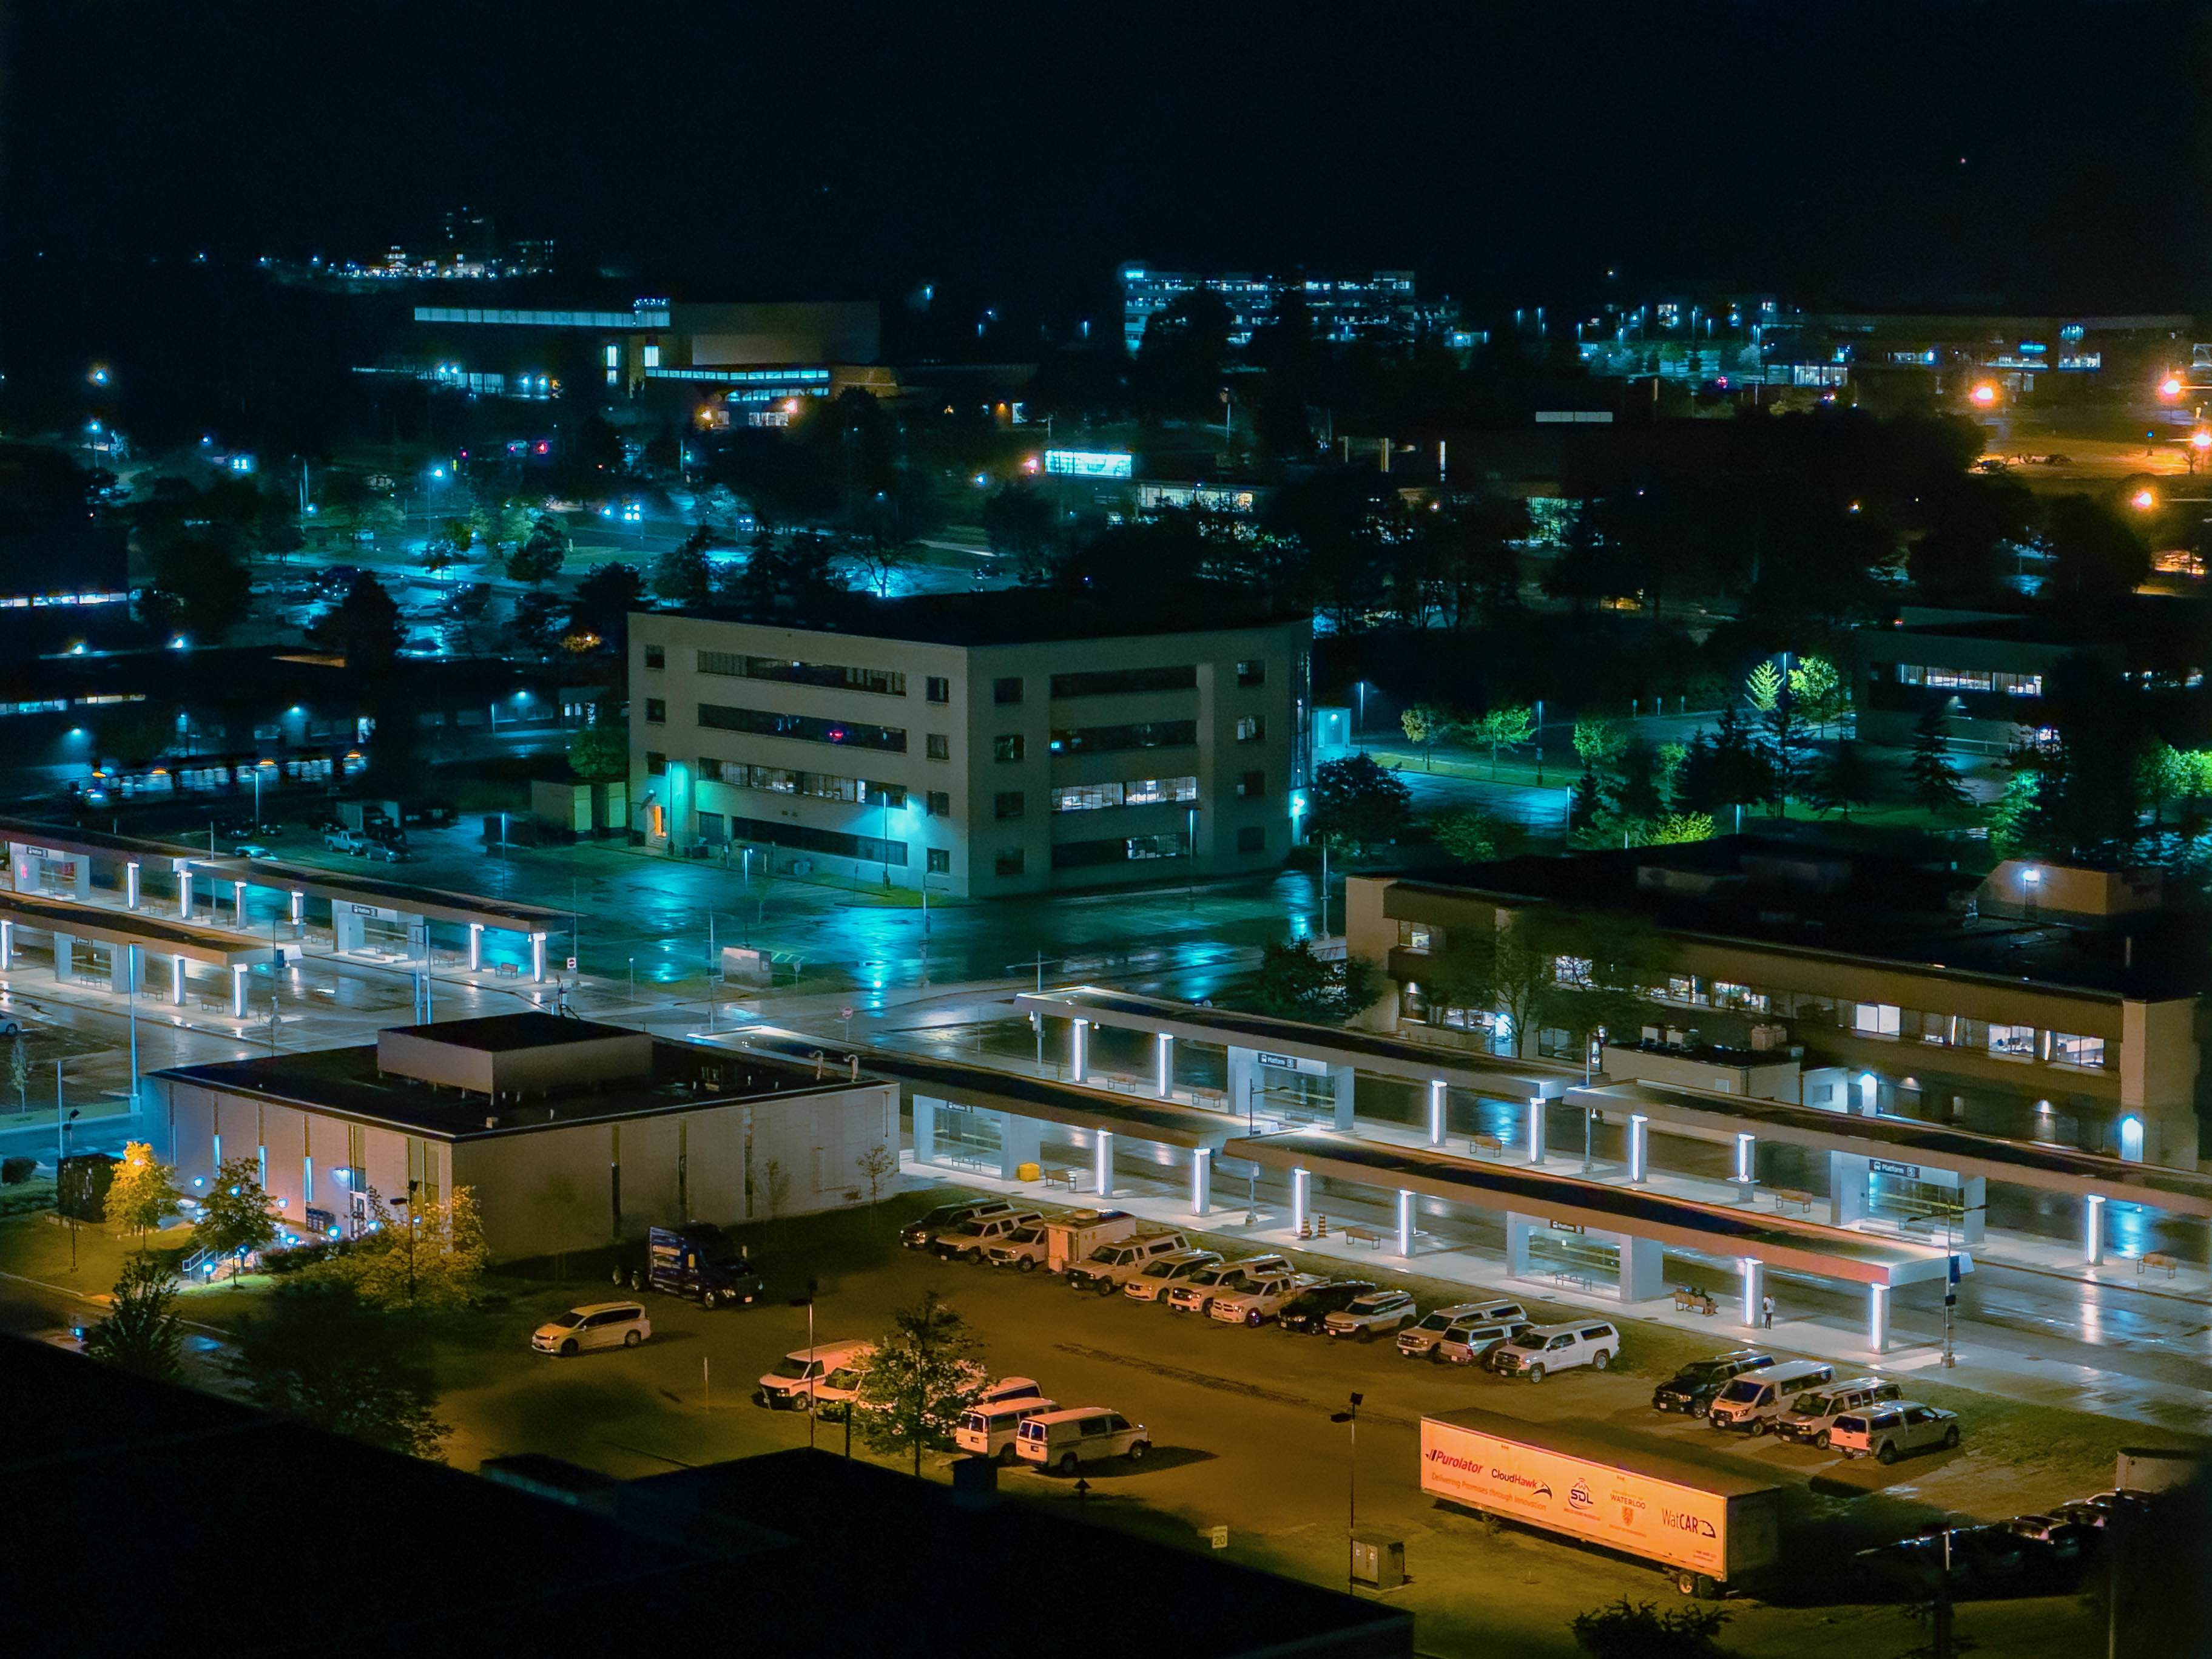
\includegraphics[scale=0.1]{img/loo.jpg}
    \caption{Waterloo, ON}
\end{figure}

\end{document}
